\chapter{OSDOCR Editor - Implementação}
\label{cap_osdocr_editor_implementacao}


% proposito e ferramentas utilizadas

Neste capítulo será analisada a implementação do último módulo da solução OSDOCR, um editor de OCR Tree gráfico. Este vem com o propósito de servir como uma outra aplicação do Toolkit criado, maioritariamente no que toca às ferramentas que rondam a estrutura OCR Tree, assim como um complemento para a OSDOCR Pipeline que, em casos mais complexos, ou para outros tipos de documentos que não foram o foco da solução, requeira uma manipulação dos resultados mais manual. O editor gráfico facilita esta manipulação.

Embora todos os níveis da OCR Tree possam ser transformados com o editor, o objetivo principal é a de trabalhar com os de nível 2, sendo este nível o que será desenhado na tela de edição.

Esta interface gráfica foi criada utilizando para a parte visual e controlo das Views as bibliotecas \textbf{PySimpleGui} e \textbf{MatplotLib}; e para módulo de dados e controlador destes o Toolkit, com a opção de utilizar a Pipeline para a realização de OCR localmente no input.


\section{Sumário}

Segue-se uma listagem das funcionalidades que serão realçadas:

\begin{itemize}\setlength\itemsep{-0.9em}
	\item Inputs
	\item Manipulação manual de OCR Tree 
	\item Aplicação local de OCR
	\item Ferramentas disponíveis
	\begin{itemize}\setlength\itemsep{-0.9em}
			\vspace{-1em}
			\item Divisão de blocos
			\item Junção de blocos
			\item Categorização de blocos
			\item Ordenação de blocos
			\item Segmentação de blocos em artigos
			\item Divisão de imagem
		\end{itemize}
	\item Outputs
	\item Operações adicionais
\end{itemize}

\section{Funcionalidades}

\subsection{Inputs}

Naturalmente, a primeira funcionalidade a ser discutida são os tipos de ficheiros de entrada necessários e admitidos pelo editor.

Sendo este um editor de OCR Tree, poderia se esperar que o único input necessário seria um ficheiro compatível com OCR Tree, no entanto, a utilidade da ferramenta seria consideravelmente limitada se o utilizador não tivesse a imagem par da OCR Tree para servir como fundo. Tomou-se então a decisão que são necessários 2 inputs para iniciar a tela de edição do GUI, uma imagem de input e um ficheiro convertível para OCR Tree - seja este um Json ou HOCR.

Realça-se que a imagem e a OCR Tree podem não corresponder, sendo responsabilidade do utilizador escolher os inputs corretamente pareados. 

A tela resultará na OCR Tree sobreposta na imagem de input. Se estes estiverem propriamente pareados, os blocos desenhados estarão corretamente alinhados com o texto respetivo na imagem.


\begin{figure}[H]
	\centering
	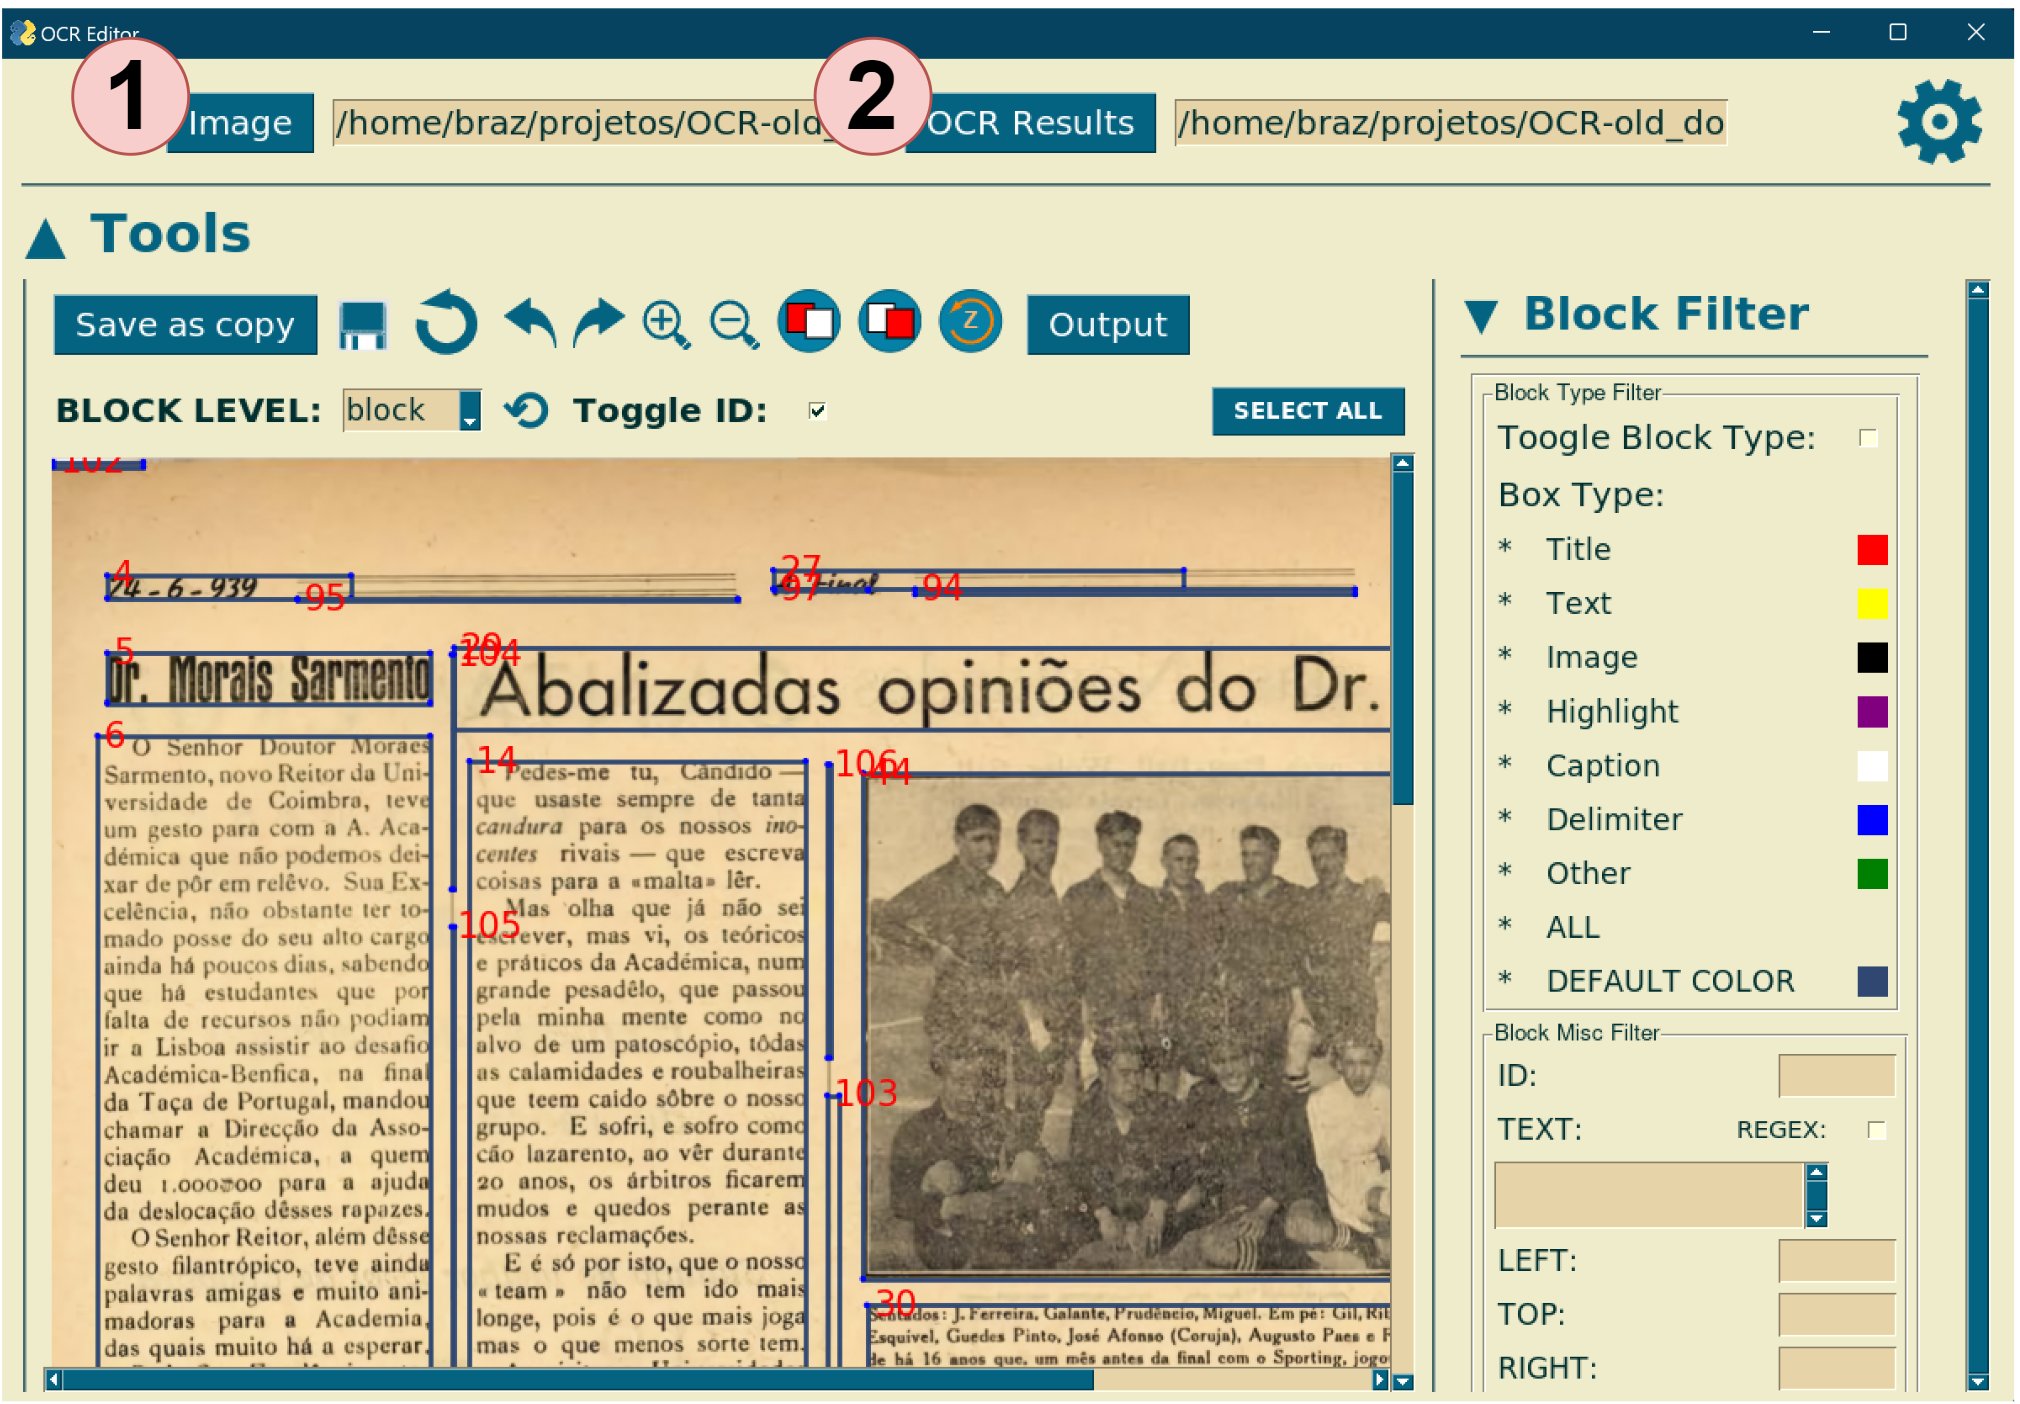
\includegraphics[width=0.7\textwidth]{images/ilustracoes/ocr_editor_inputs.png}
	\caption{OCR Editor: escolha de inputs. 1 - Input de imagem. 2 - Input de ficheiro OCR Tree}
	\label{fig:ocr_editor_inputs}
\end{figure}



Numa nota extra sobre os inputs: o editor possui uma opção nas configurações que permite que ao ser escolhida uma imagem de input, seja procurada automaticamente por outputs desta resultantes do uso da pipeline, acelerando o processo de seleção da OCR Tree.


\subsection{Manipulação manual de OCR Tree}

Segue-se o propósito principal da criação do editor gráfico, a facilitação da manipulação manual de OCR Tree.

Utilizando o OSDOCR Editor é possível:

\textbf{Selecionar blocos} clicando nestes usando o rato. Múltiplos blocos podem ser selecionados - mantendo premido a tecla 'ctrl' ou clicando e arrastando por cima de uma área -  e, consequentemente, manipulados em simultâneo. Para desselecionar um bloco, basta clicar neste novamente ou selecionar uma zona sem blocos.

\begin{figure}[H]
	\centering
	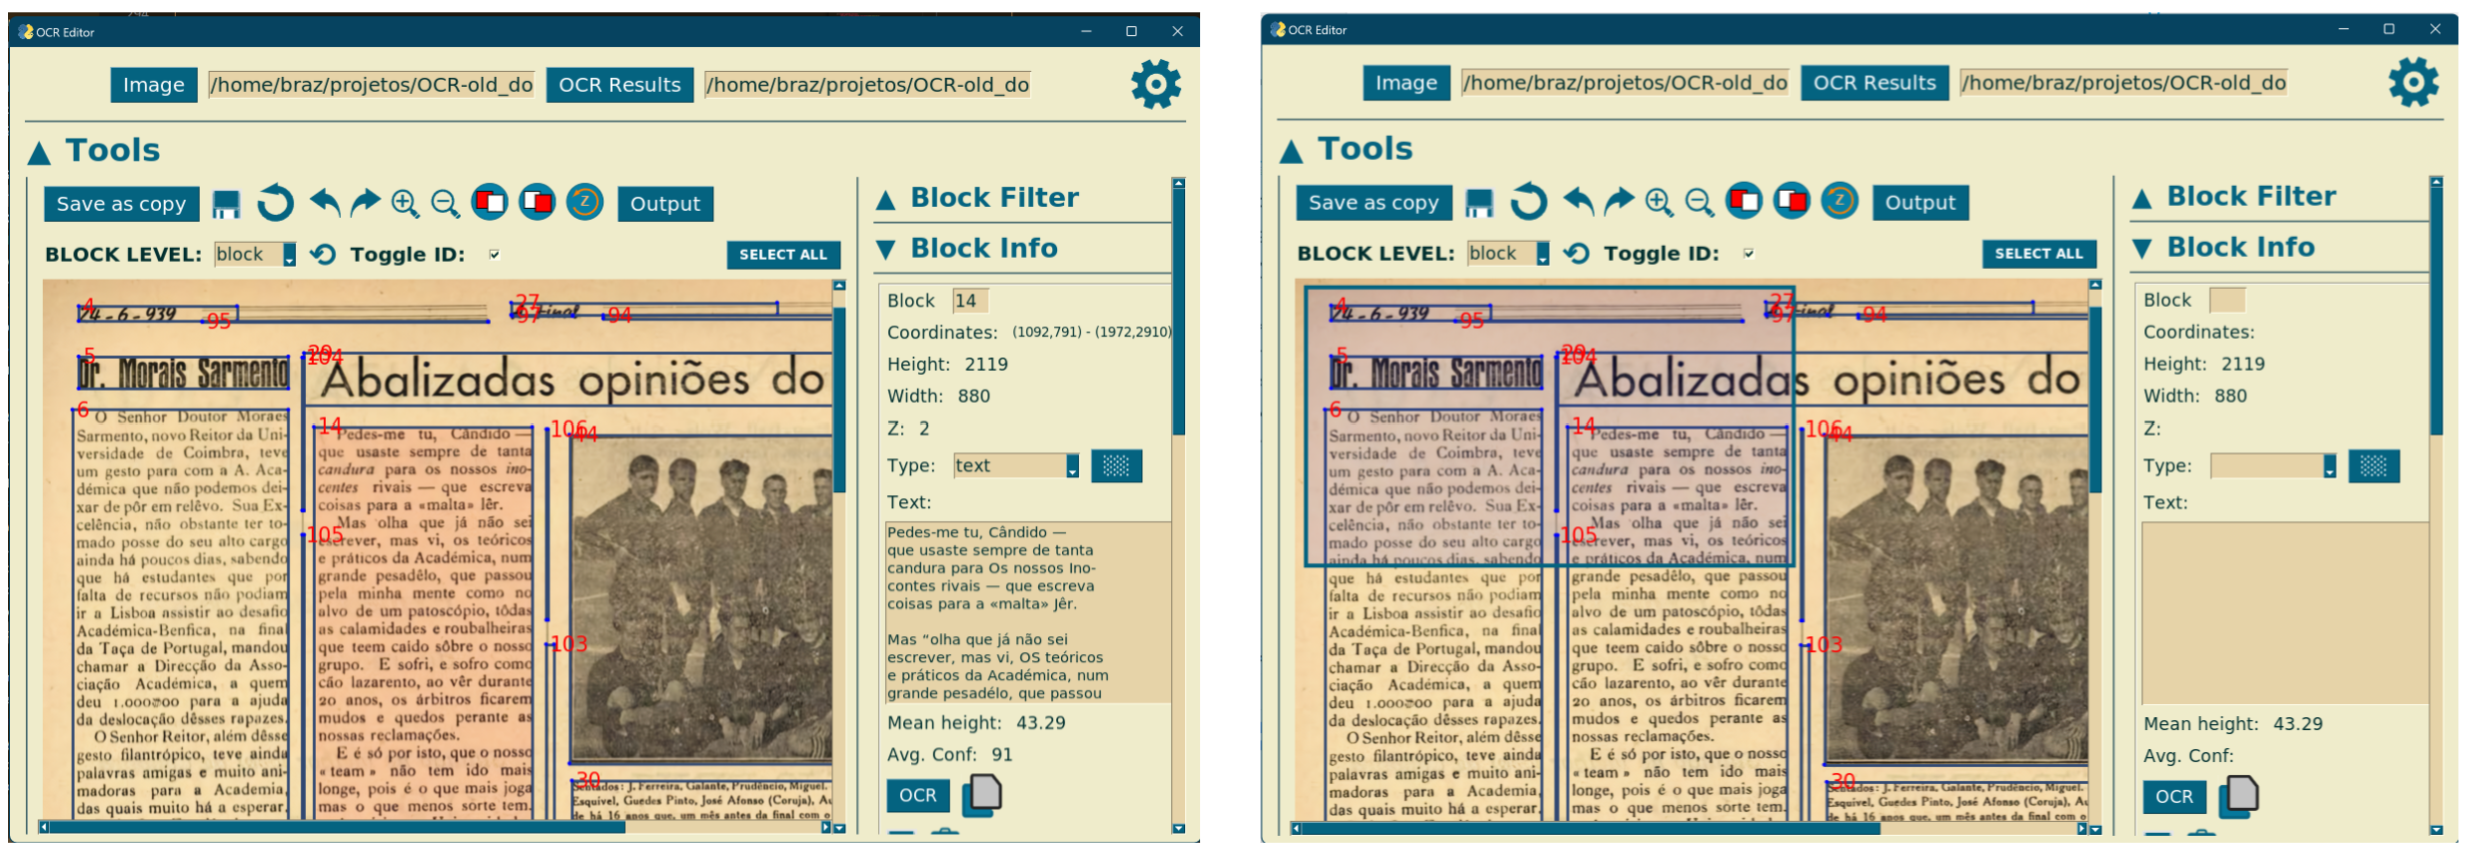
\includegraphics[width=1.1\textwidth]{images/ilustracoes/ocr_editor_select.png}
	\caption{OCR Editor: seleção de blocos}
	\label{fig:ocr_editor_select}
\end{figure}


\textbf{Mover blocos} selecionando um ou múltiplos blocos e, com o botão do rato pressionado, mover o cursor para o local desejado.

\begin{figure}[H]
	\centering
	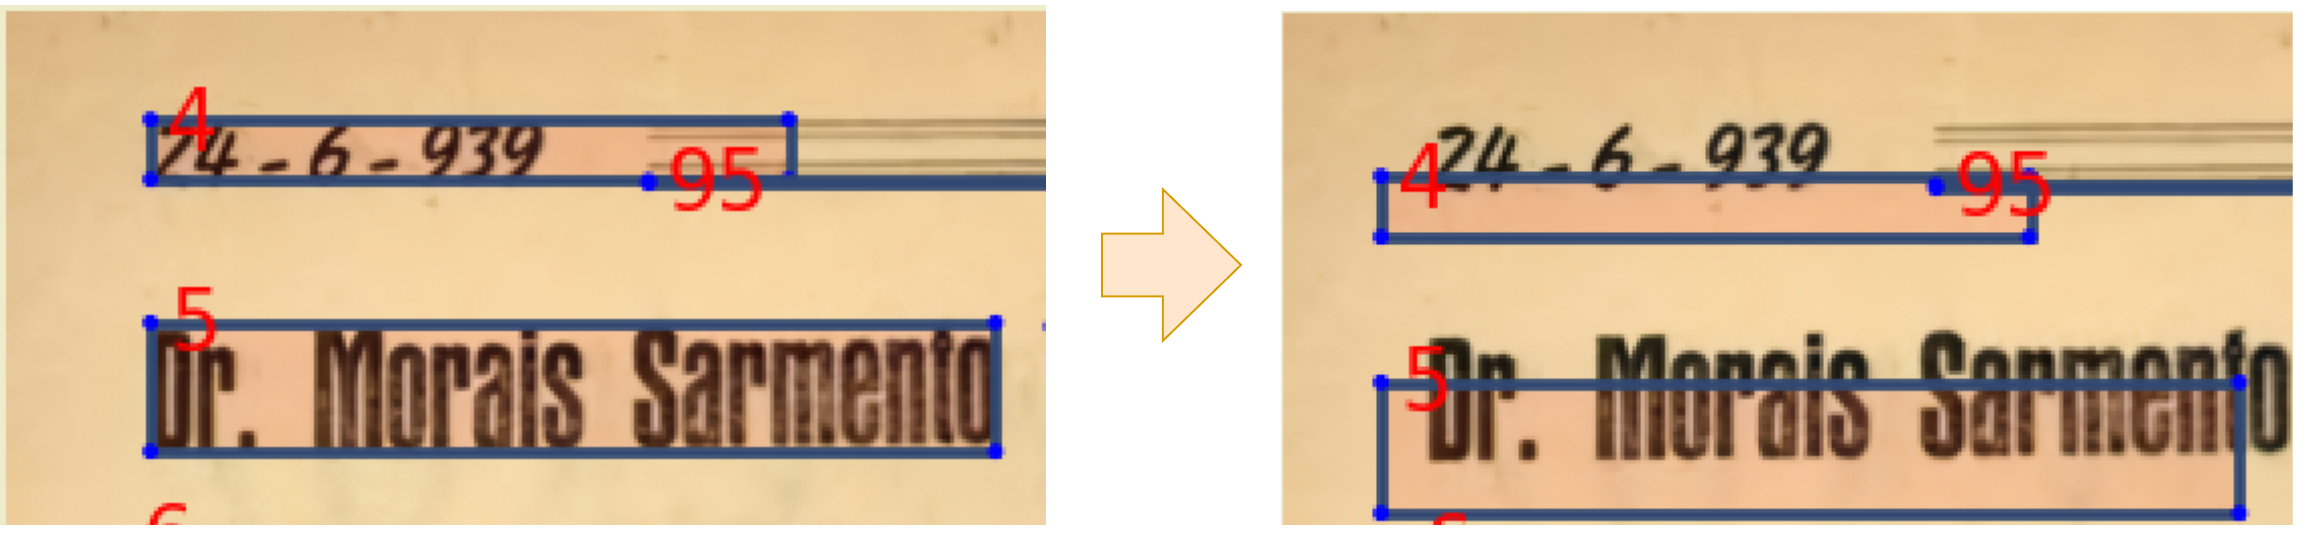
\includegraphics[width=0.5\textwidth]{images/ilustracoes/ocr_editor_move.png}
	\caption{OCR Editor: mover blocos}
	\label{fig:ocr_editor_move}
\end{figure}


\textbf{Redimensionar blocos} selecionando um ou múltiplos blocos e, clicando no vértice para pivô de redimensionamento, mover conforme desejado.

\begin{figure}[H]
	\centering
	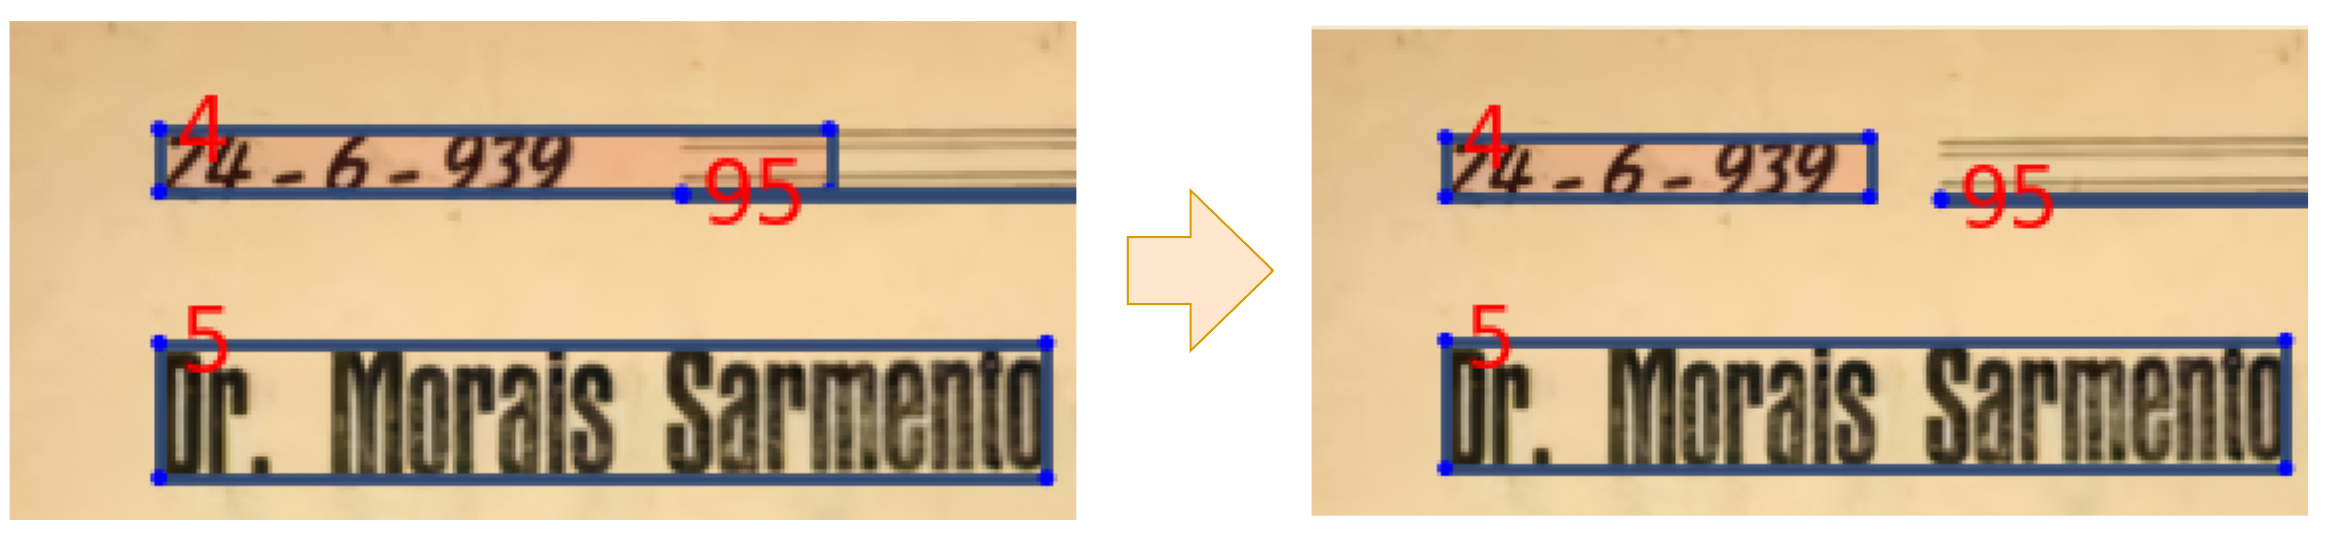
\includegraphics[width=0.5\textwidth]{images/ilustracoes/ocr_editor_resize.png}
	\caption{OCR Editor: redimensionar bloco}
	\label{fig:ocr_editor_resize}
\end{figure}

\textbf{Atualizar texto do bloco} manualmente, ao selecionar um bloco e, na aba da direita com a informação do bloco, atualizar o texto de acordo e clicar em salvar. No caso de múltiplos blocos serem selecionados, apenas o último selecionado é modificável.

Realça-se que a edição manual do texto leva a perda de alguma informação, nomeadamente as dimensões dos níveis mais profundos dentro do bloco, visto que requerer ao utilizador que delimite as coordenadas e nível de confiança de texto das linhas, palavras ou parágrafos editados iria contra o propósito da edição de OCR Tree facilitada. Estes níveis terão aos suas dimensões repartidas de forma uniforme de forma a encaixarem dentro do bloco pai e a confiança de texto será considerada como total (100).

\begin{figure}[H]
	\centering
	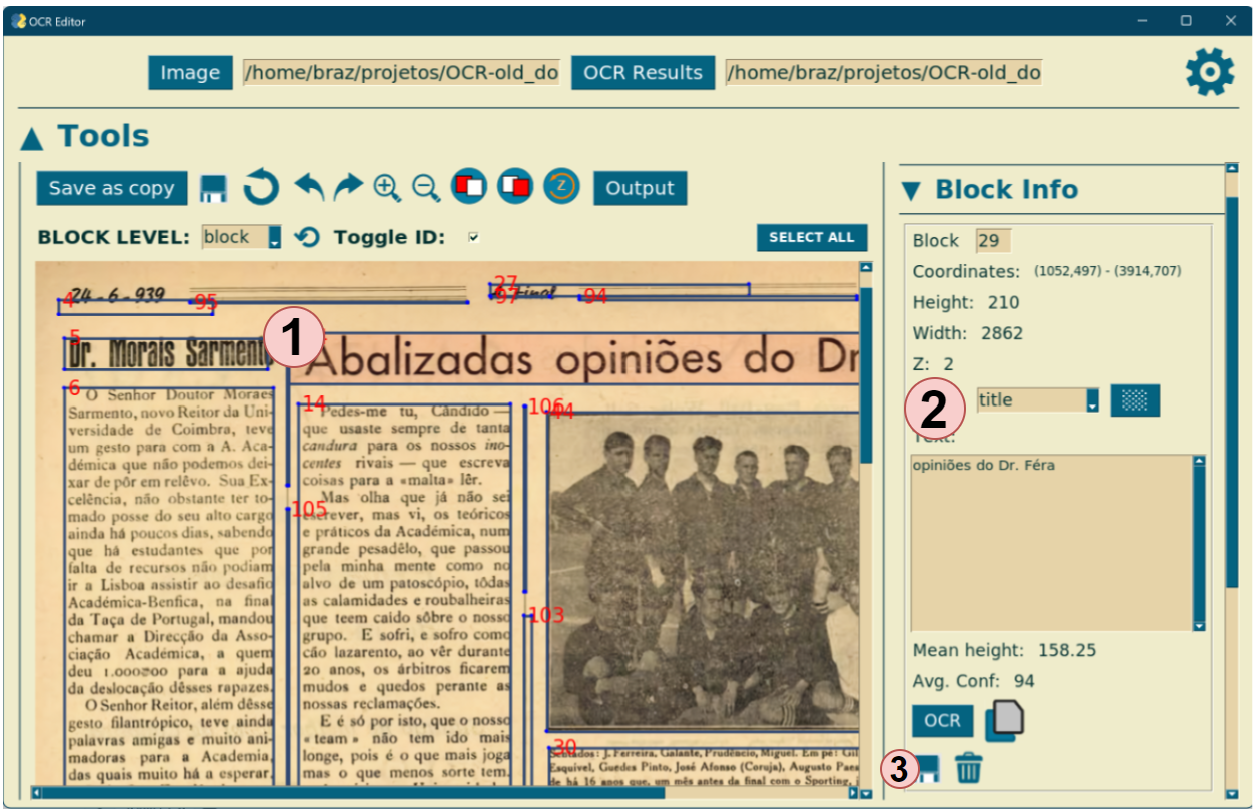
\includegraphics[width=0.7\textwidth]{images/ilustracoes/ocr_editor_update.png}
	\caption{OCR Editor: atualizar bloco. 1 - Selecionar bloco. 2 - Modificar dados do bloco. 3 - Guardar alterações.}
	\label{fig:ocr_editor_update}
\end{figure}

\textbf{Adicionar um novo bloco} clicando no botão do meio do rato no local desejado, ou utilizando o botão com o mesmo efeito.

\begin{figure}[H]
	\centering
	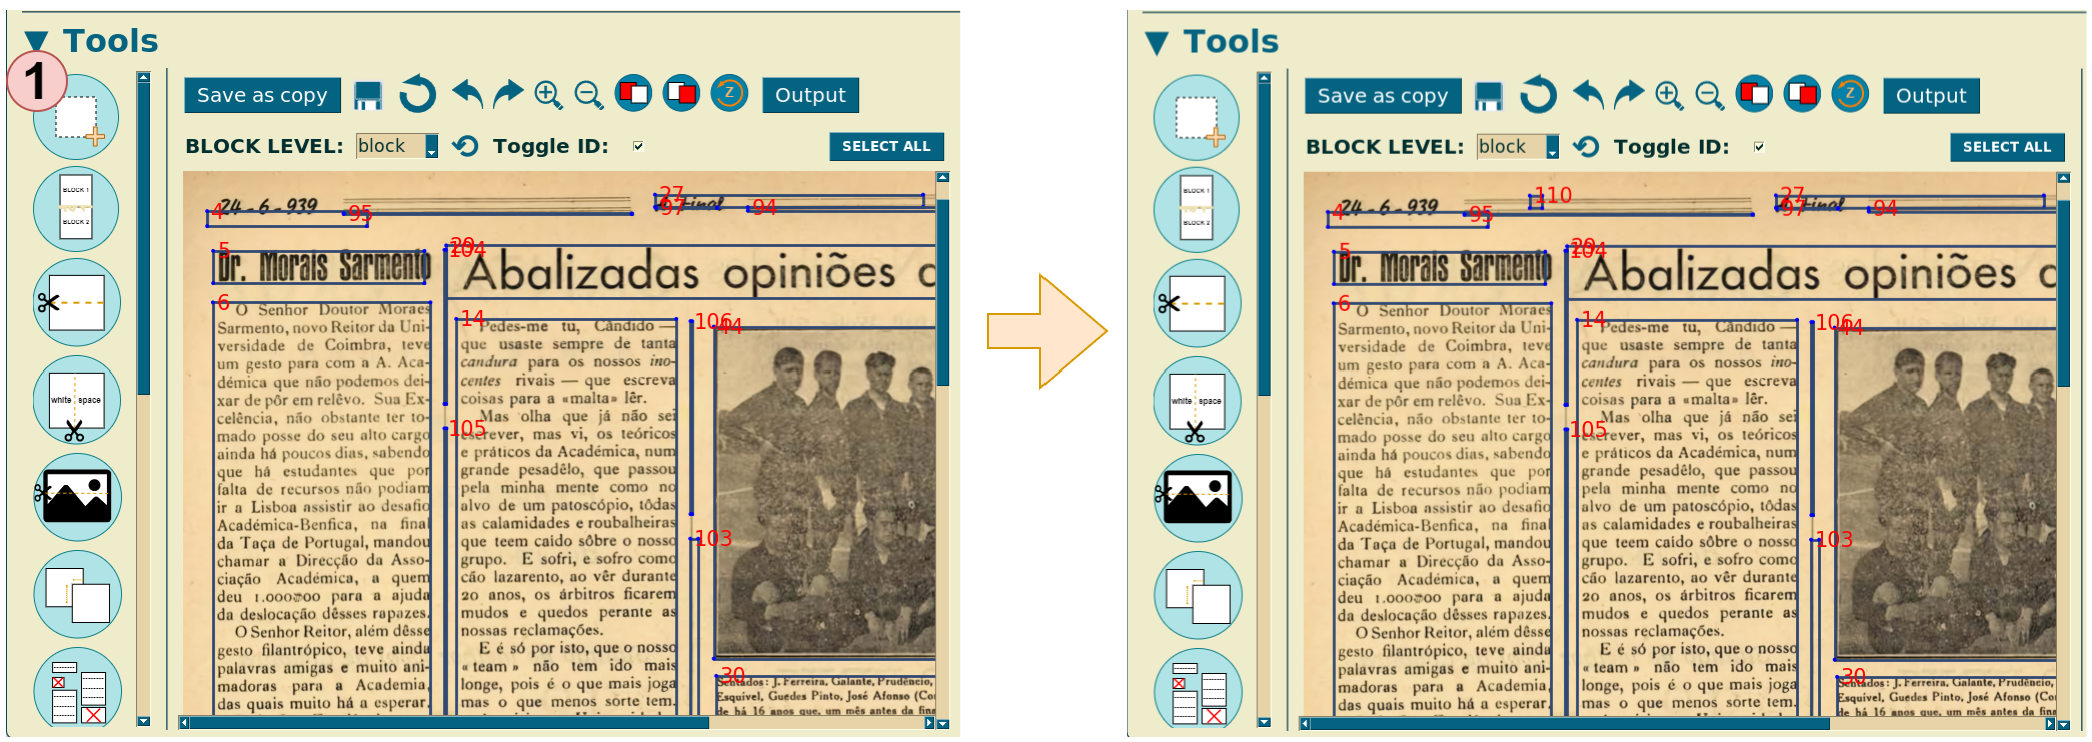
\includegraphics[width=1\textwidth]{images/ilustracoes/ocr_editor_new_block.png}
	\caption{OCR Editor: criar novo bloco. 1 - Ferramenta para criar novo bloco (ID 110).}
	\label{fig:ocr_editor_new_block}
\end{figure}


\textbf{Remover um bloco} selecionando o bloco a remover e clicando no botão (ou utilizando a tecla 'delete') para o efeito. No caso de múltiplos blocos selecionados, todos serão removidos.

\begin{figure}[H]
	\centering
	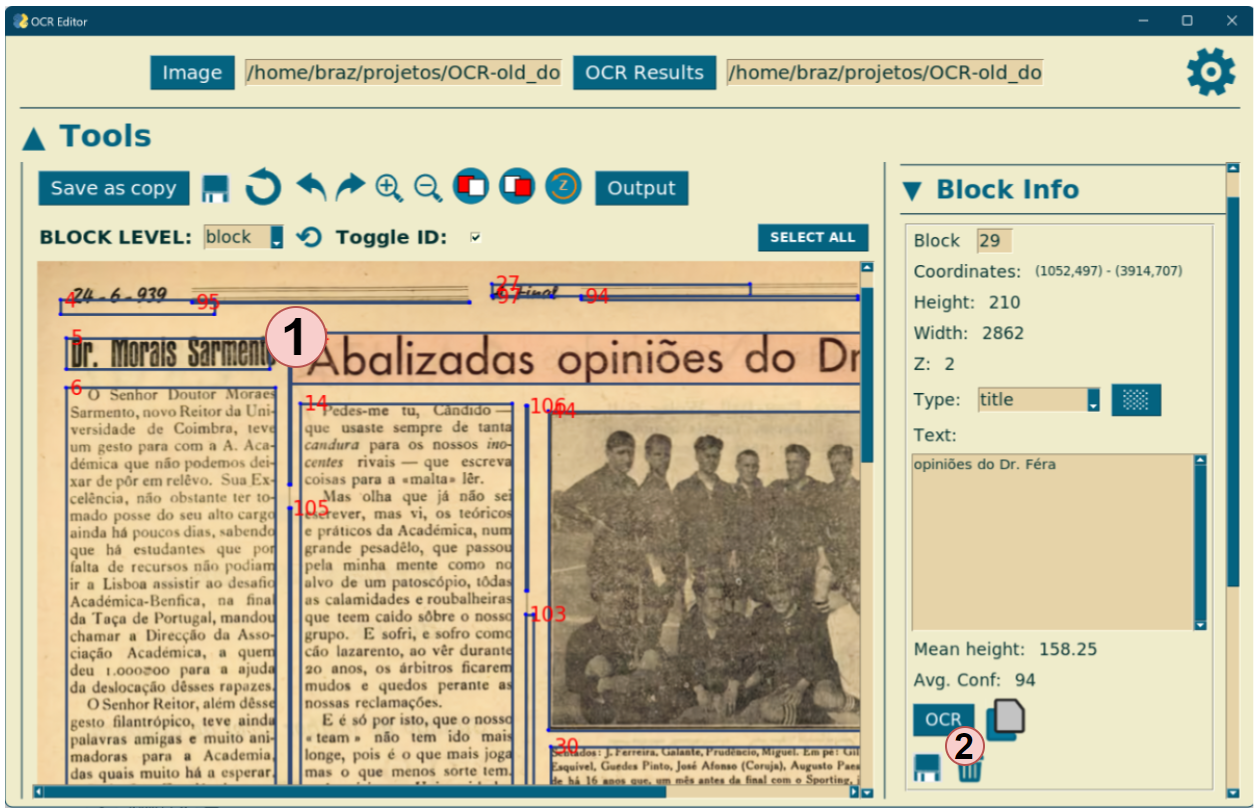
\includegraphics[width=0.7\textwidth]{images/ilustracoes/ocr_editor_delete_block.png}
	\caption{OCR Editor: eliminar bloco. 1 - Selecionar bloco. 2 - Eliminar bloco.}
	\label{fig:ocr_editor_delete_block}
\end{figure}



\subsection{Aplicação local de OCR}

Em instâncias em que apenas porções da OCR Tree apresentem resultados não satisfatórios, ou se pretenda criar novos blocos de texto, a habilidade de aplicar OCR no local afetado é mais prática do que transcrever o texto manualmente por completo.

Isto consegue-se aplicando a OSDOCR Pipeline. Nas configurações do editor é possível costumizar os parâmetros da pipeline a utilizar, por exemplo: não aplicar pós processamento e no pré processamento não realizar upscaling.

A utilização da implementação da pipeline implica que é necessário transformar os outputs desta, transformando a OCR Tree resultante numa de nível 2 e, atualizar as suas coordenadas para fazerem sentido à posição do bloco no input do editor, assim como a escala das dimensões caso necessário.

Uma configuração própria desta funcionalidade, é a escolha entre os resultados serem comprimidos em um único bloco, ou serem inseridos novos blocos de acordo com os resultados da pipeline. Deste modo, é também possível realizar OCR numa imagem inteira, ampliando esta ferramenta.

Para utilizar esta funcionalidade própria do editor, basta selecionar o bloco alvo e clicar no botão de OCR na aba lateral direita.


\begin{figure}[H]
	\centering
	\hspace*{-1.8cm}
	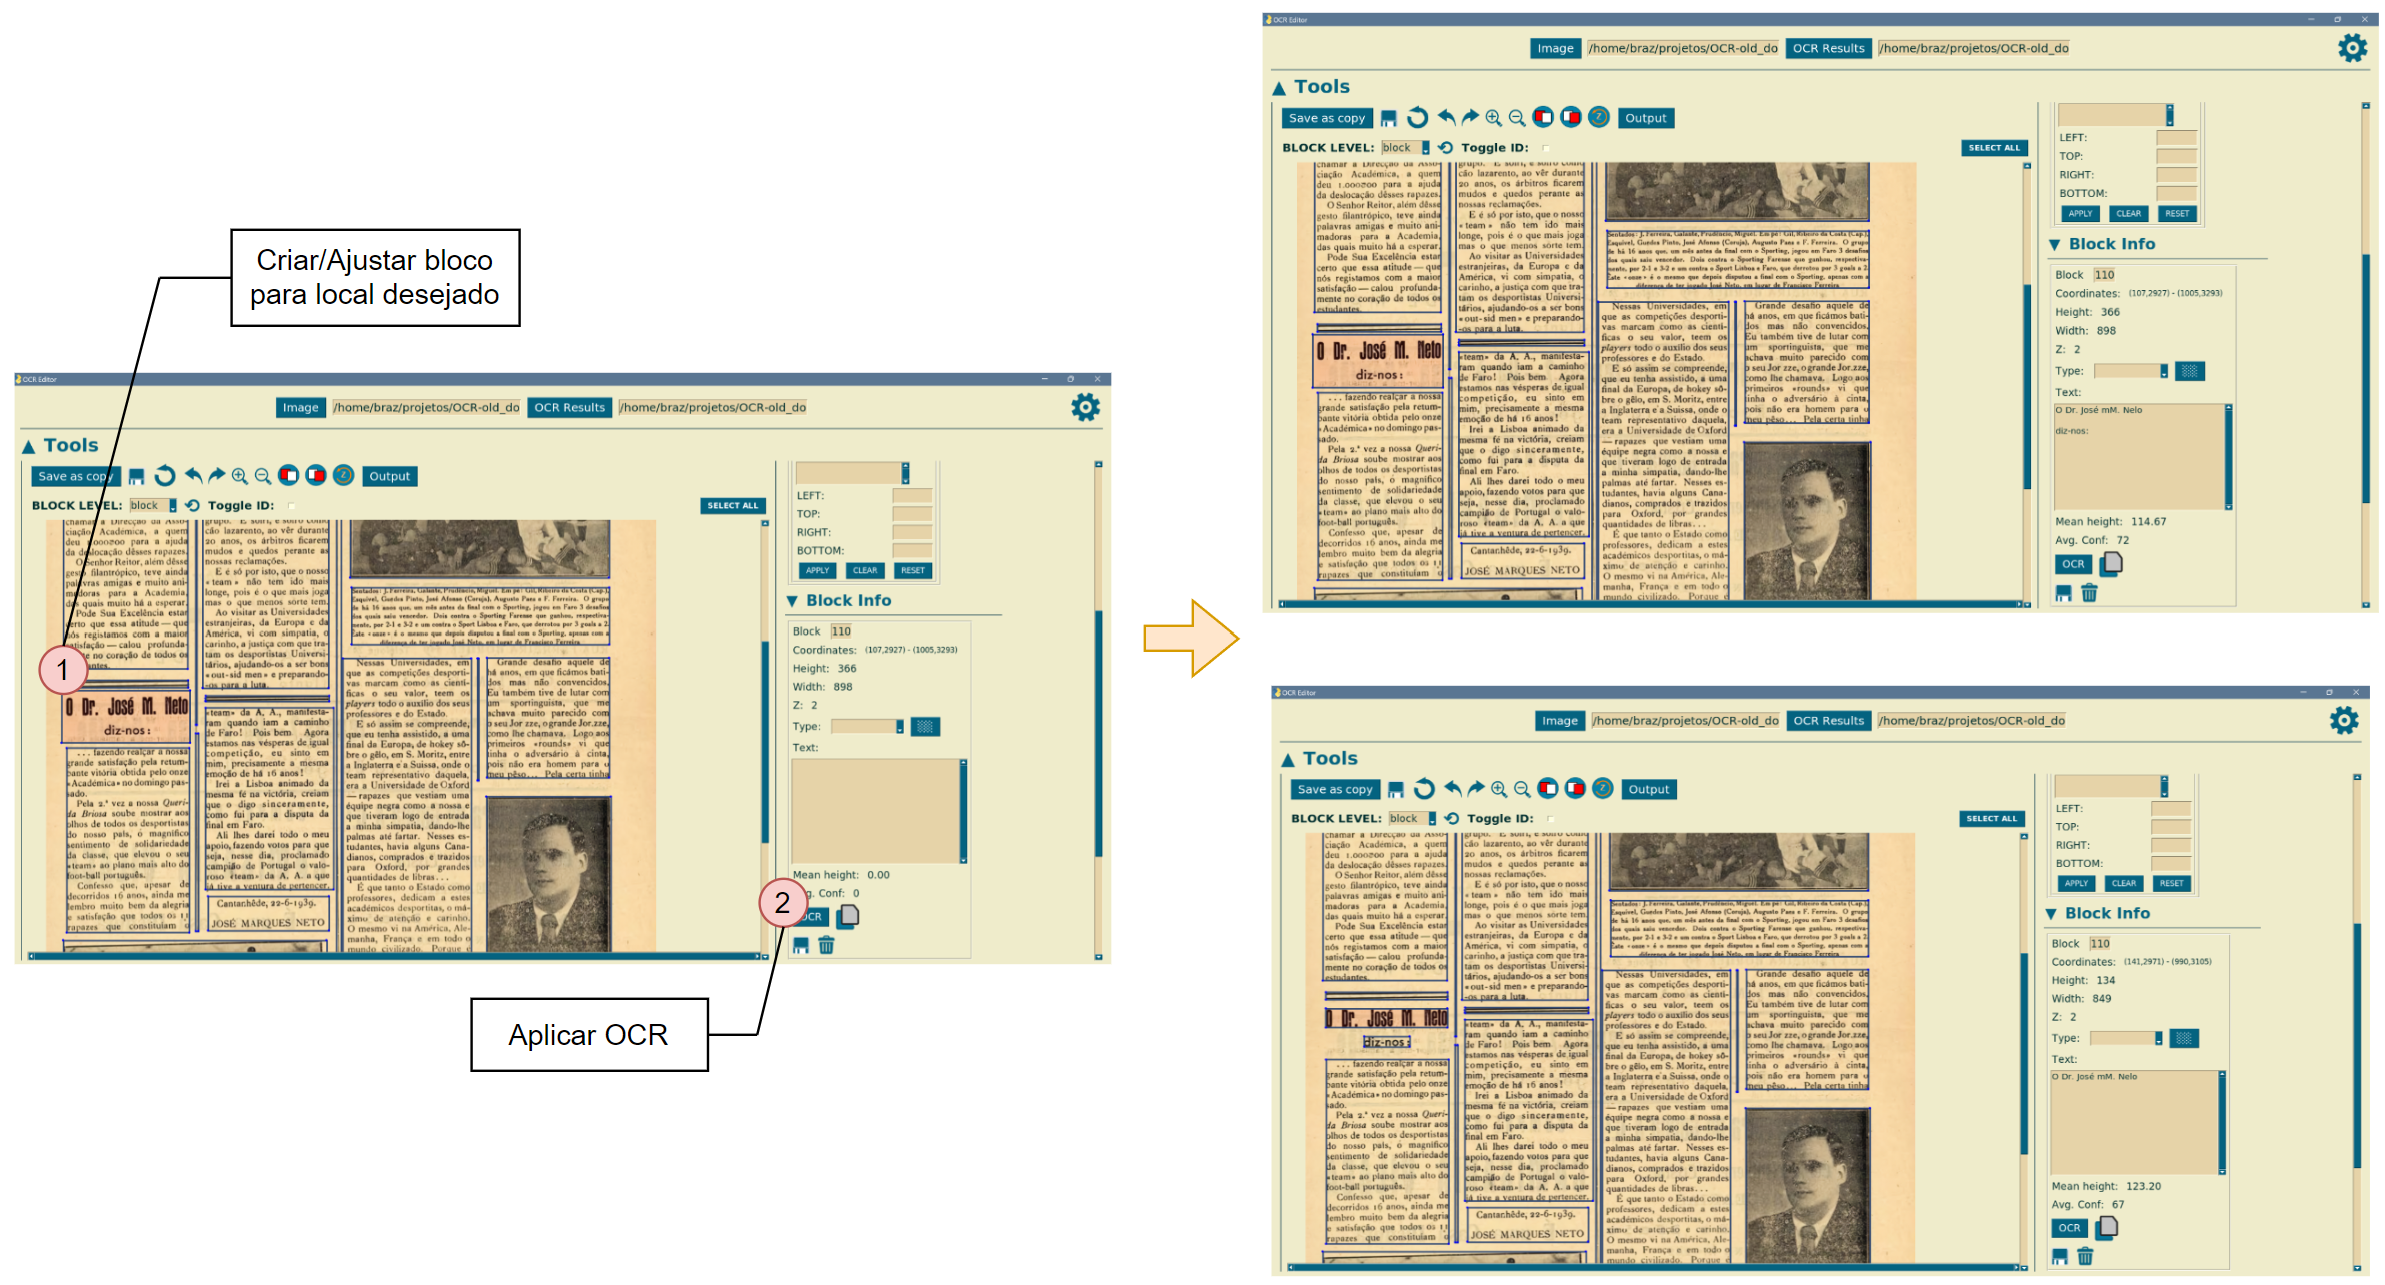
\includegraphics[width=1.2\textwidth]{images/ilustracoes/ocr_editor_apply_ocr.png}
	\caption{OCR Editor: aplicar OCR. 1 - Selecionar bloco. 2 - Aplicar OCR. Resultado em cima - bloco único. Resultado em baixo - blocos resultantes.}
	\label{fig:ocr_editor_apply_ocr}
\end{figure}




\subsection{Ferramentas disponíveis}

Nesta secção serão descritas as funcionalidades conseguidas através do uso do OSDOCR Toolkit. Várias destas já estão presentes no OSDOCR pipeline porém, o editor permite uma utilização mais controlada destas.

\highlight{Divisão de blocos}

A divisão de blocos tem como principal propósito corrigir a segmentação de blocos realizada pelo motor OCR.

Nesta categoria temos 2 tipos de divisão:

\highlight{Corte de bloco}[\normalsize]

Esta funcionalidade não está diretamente disponível na pipeline - embora o toolkit a ofereça e outras funcionalidades na pipeline façam uso deste método - devido a necessitar de um input humano.

Tendo selecionado um bloco para realizar um corte e, em seguida, clicado na funcionalidade de corte, o editor irá entrar no estado especial de recorte. Este é caracterizado por uma linha de corte aparecer sob o bloco selecionado, servindo como auxílio para a divisão do bloco em 2.


Clicando no botão esquerdo do rato neste estado realizará o corte de acordo com a linha visível. O texto será também divido entre os dois blocos de acordo com a linha de corte escolhida. Naturalmente, a divisão do texto segue na realidade as coordenadas da linha de corte e da OCR Tree respetiva ao bloco, sendo que se a bounding box não estiver propriamente alinhada com o texto respetivo, esta divisão poderá não fazer sentido visualmente.

\begin{figure}[H]
	\centering
	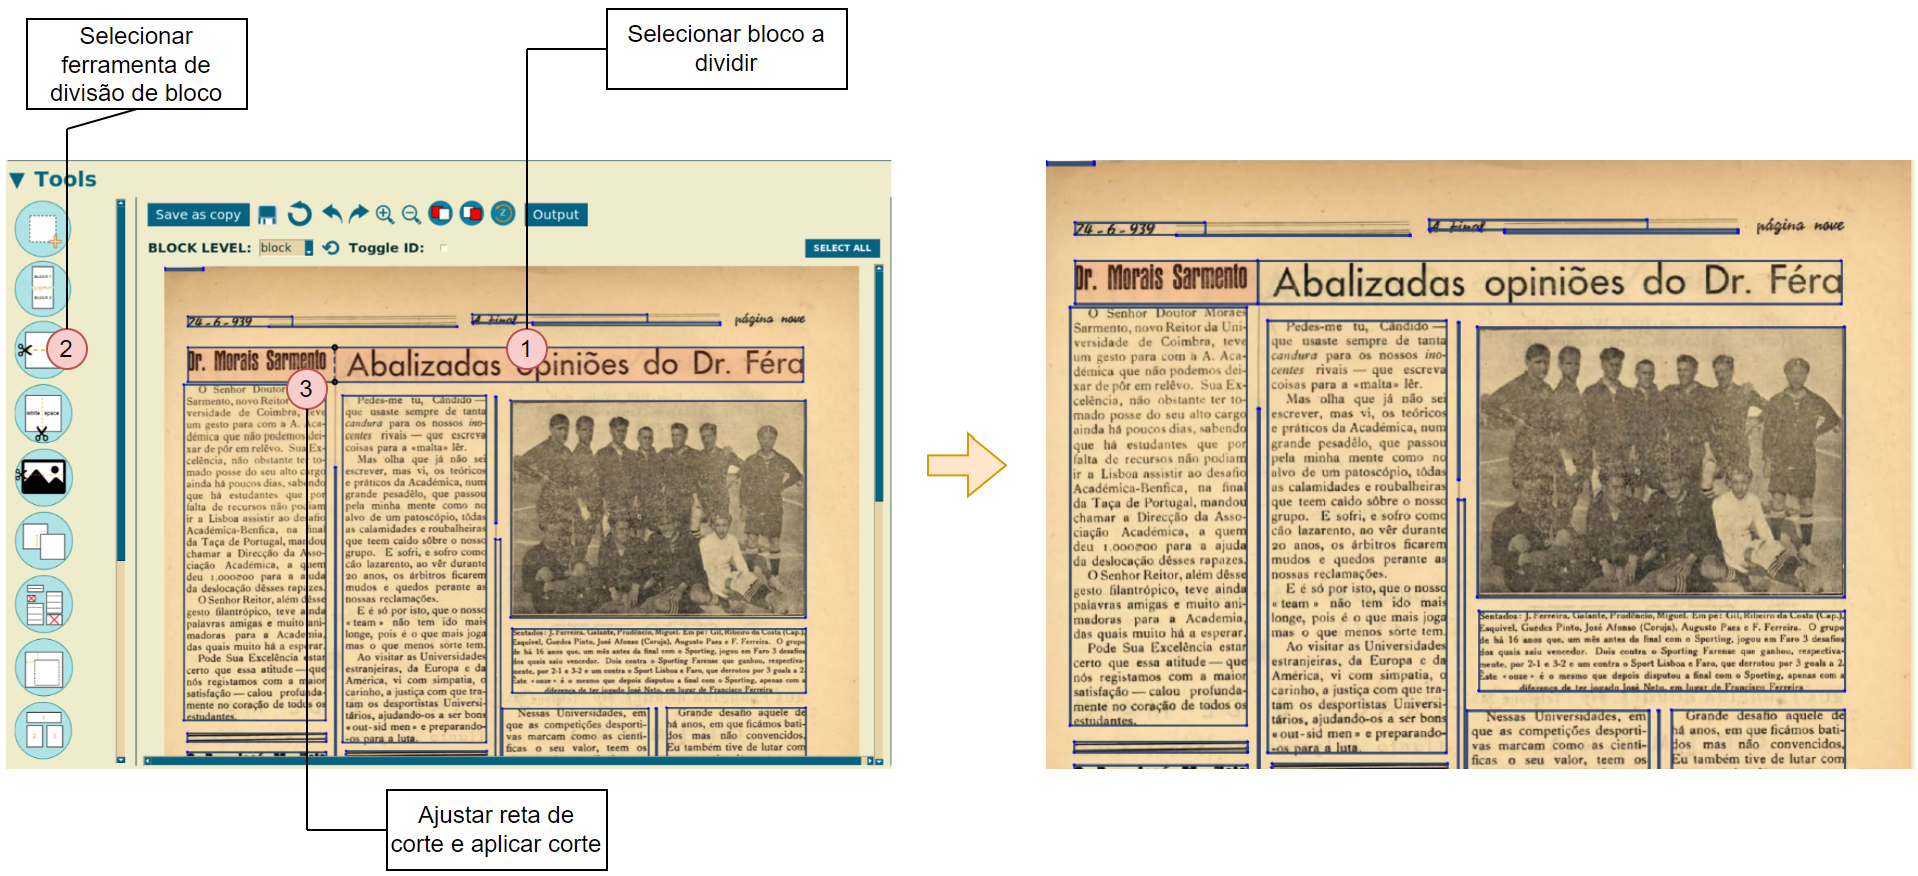
\includegraphics[width=1\textwidth]{images/ilustracoes/ocr_editor_split_block.png}
	\caption{OCR Editor: divisão de bloco.}
	\label{fig:ocr_editor_split_block}
\end{figure}



\highlight{Divisão por espaços vazios}[\normalsize]

Esta funcionalidade é semelhante à disponibilizada na pipeline com o mesmo nome, que por sua vez provém do toolkit.

A distinção principal neste cenário é que pode ser utilizada num ambiente mais controlado, apenas afetando, caso desejado, os blocos selecionados.

Caso nenhum bloco esteja selecionado, todos os blocos serão afetados.

Devido à característica de análise estatística do algoritmo para verificação das razões dos espaços vazios, mesmo no caso de haverem blocos selecionados, será introduzido no método a OCR Tree geral.



\highlight{Junção de blocos}

Utilizando métodos de junção de múltiplas OCR Tree, tal como na pipeline no bloco de união de blocos, esta é uma utilização manual de junção de blocos.

Existem, como discutido no Toolkit, duas formas principais de junção de blocos, horizontal ou vertical.

No caso do Editor, basta selecionar dois ou mais blocos para junção e clicar na ferramenta. O algoritmo de junção irá automaticamente unir os dois textos tendo em conta as suas coordenadas, podendo ficar com linhas intercaladas.

\begin{figure}[H]
	\centering
	\hspace*{-1.8cm}
	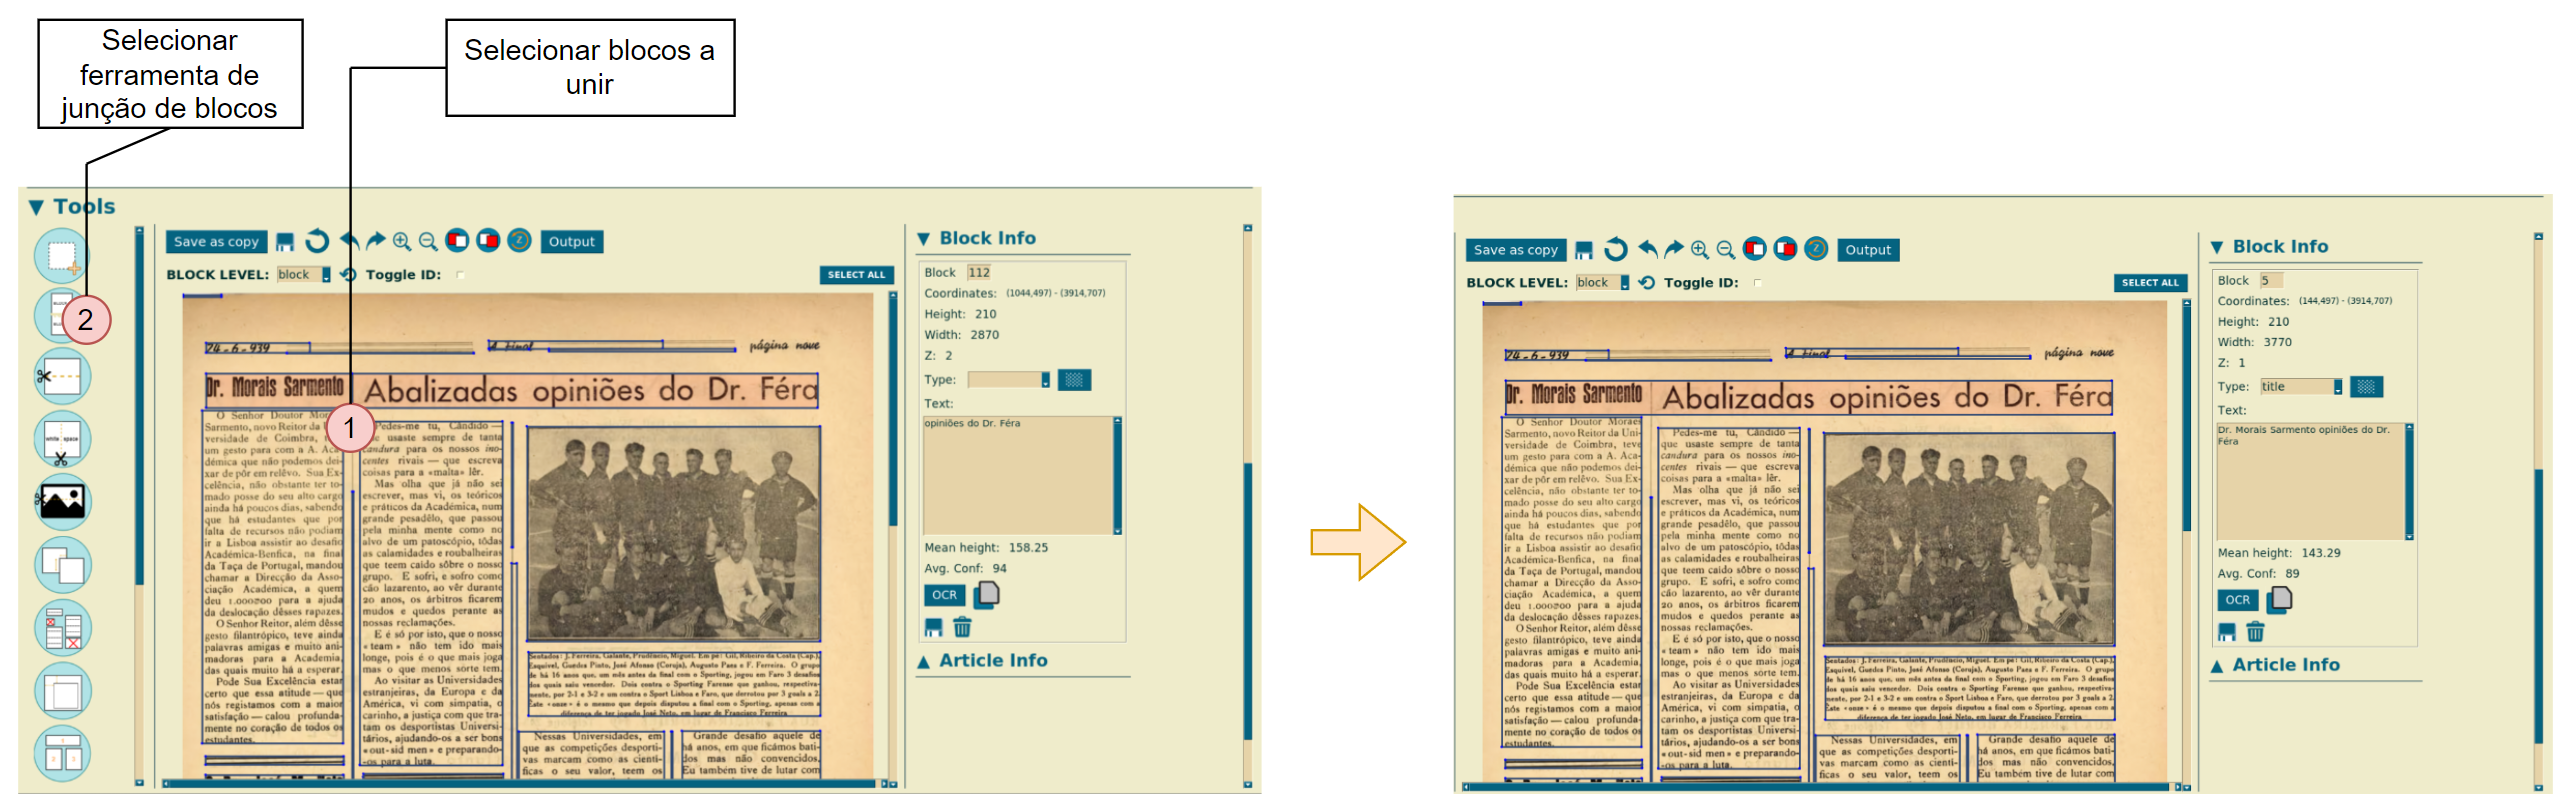
\includegraphics[width=1.2\textwidth]{images/ilustracoes/ocr_editor_join_blocks.png}
	\caption{OCR Editor: junção de bloco.}
	\label{fig:ocr_editor_join_blocks}
\end{figure}

\begin{figure}[H]
	\centering
	\hspace*{-1.8cm}
	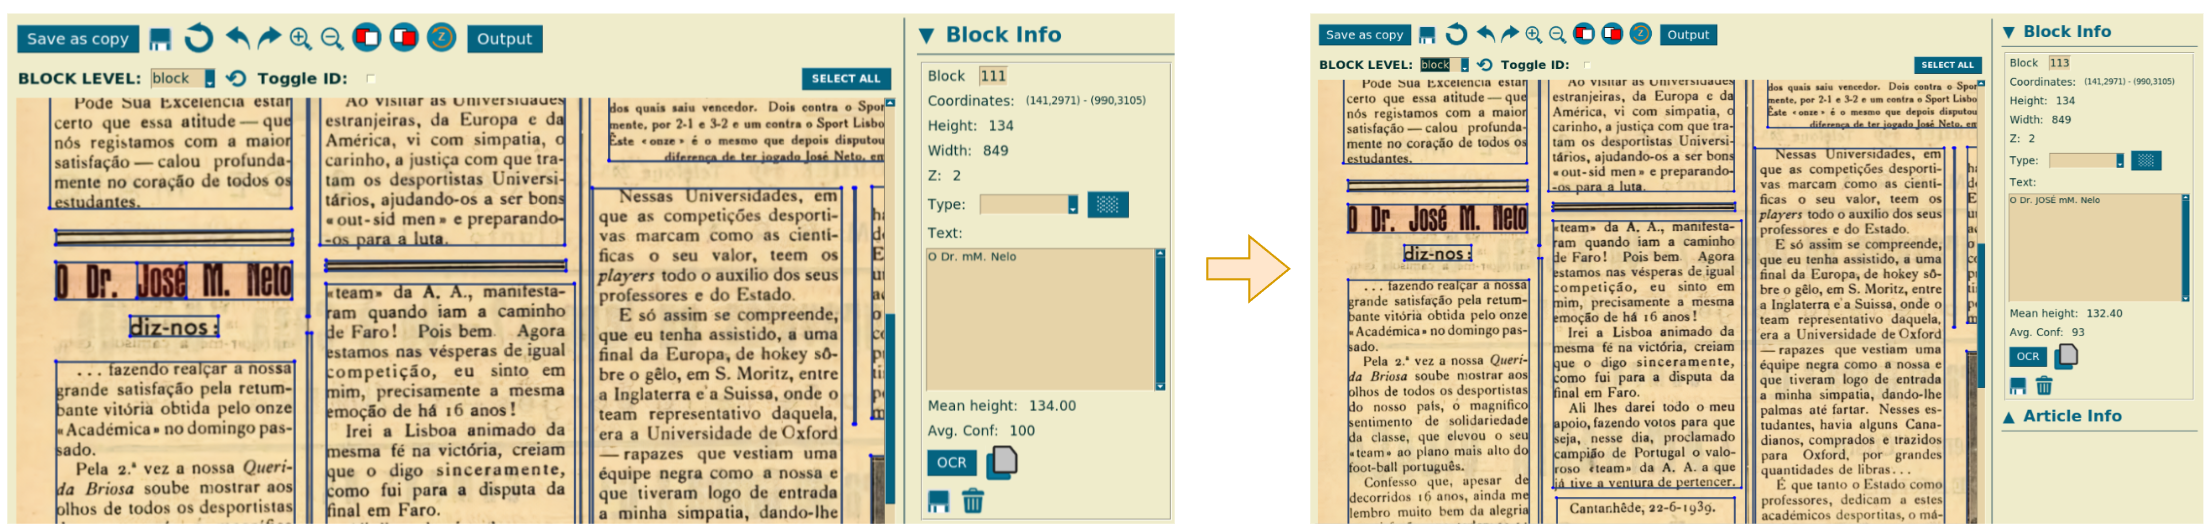
\includegraphics[width=1.2\textwidth]{images/ilustracoes/ocr_editor_join_blocks_2.png}
	\caption{OCR Editor: junção de bloco, texto intercalado. Neste exemplo foi removida a palavra "José" do bloco, e criado um novo bloco com essa mesma palavra; posicionou-se o novo bloco na posição pretendida; juntou-se os blocos.}
	\label{fig:ocr_editor_join_blocks_2}
\end{figure}


\highlight{Categorização de blocos}

A tokenização dos blocos é especialmente importante para os algoritmos de cálculo de atração entre blocos e consequentemente cálculo de ordem de leitura; e de divisão dos blocos de texto em artigos.

Desta forma, a possibilidade de realizar uma categorização manual, para maior confiança ou correções em relação ao algoritmo automático, é evidentemente benéfico.

Tal pode ser conseguido selecionando um bloco e, na aba de edição do bloco, escolher o tipo deste. Por fim, é necessário clicar para guardar as modificações no bloco.

Por defeito, o editor não ilustra os tipos dos blocos, sendo necessário escolher a opção para os diferentes tipos de blocos serem coloridos.

\begin{figure}[H]
	\centering
	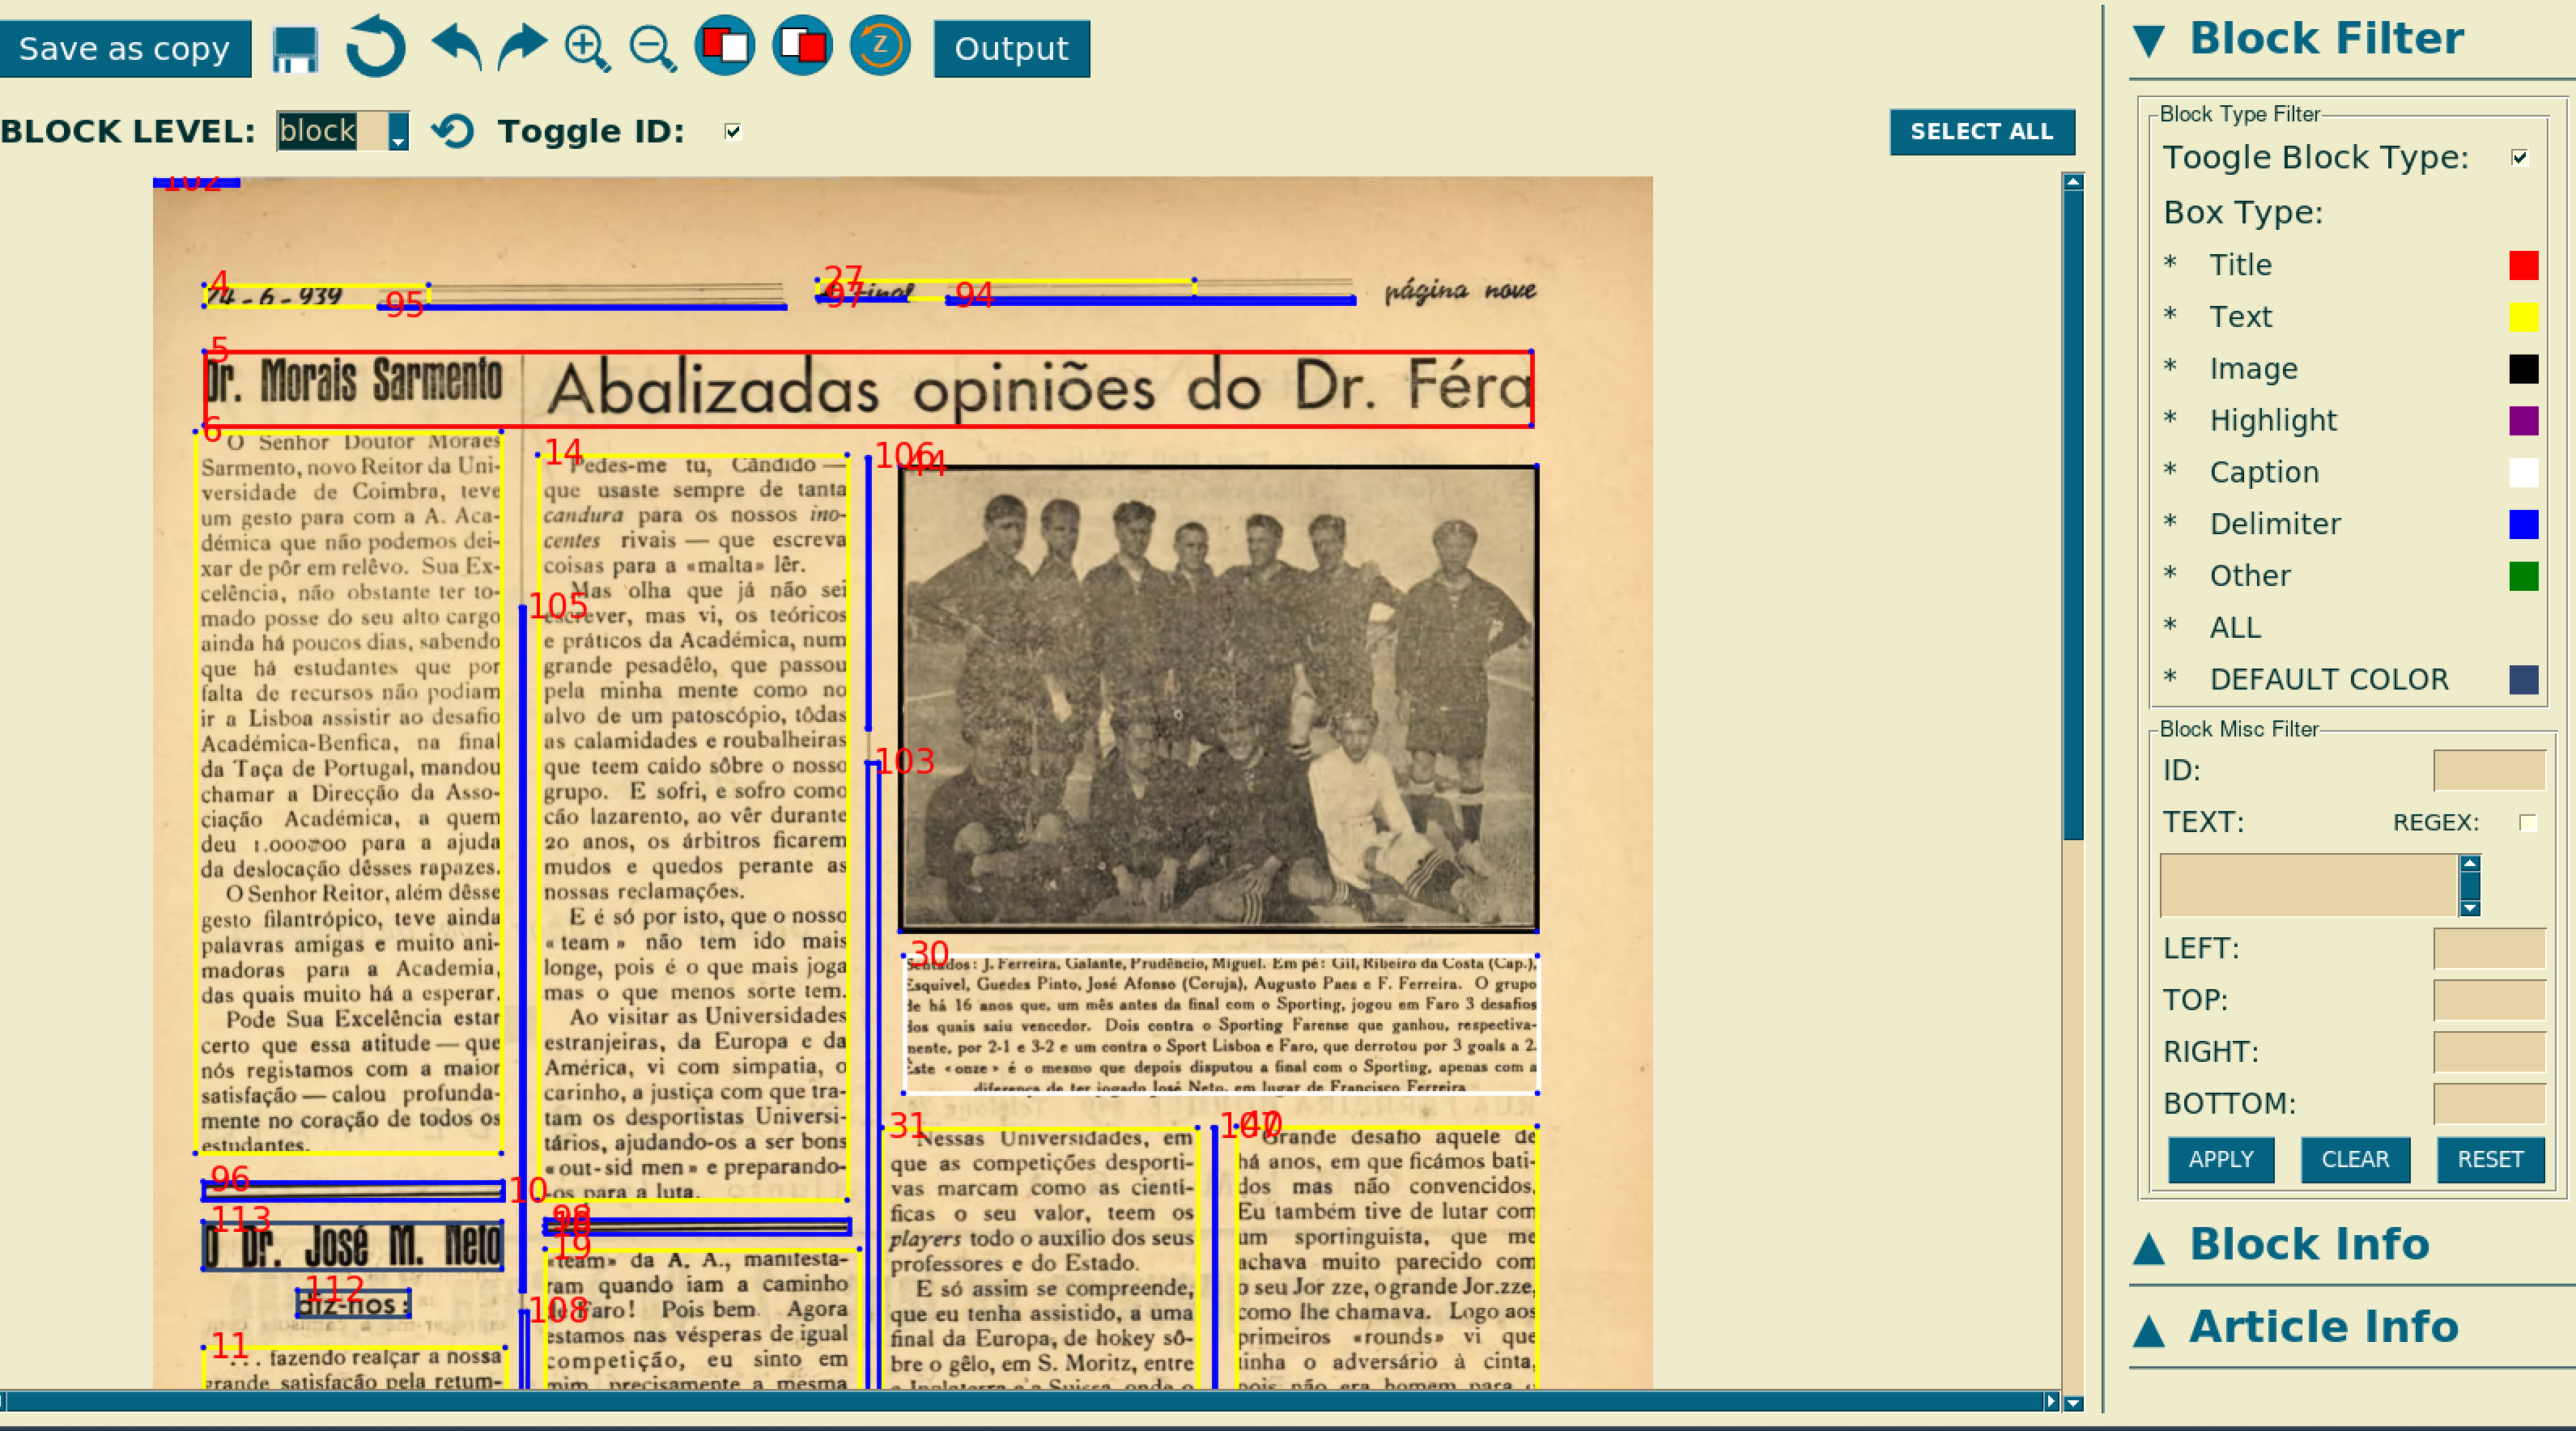
\includegraphics[width=0.6\textwidth]{images/ilustracoes/ocr_editor_block_types.png}
	\caption{OCR Editor: categorização de blocos.}
	\label{fig:ocr_editor_block_types}
\end{figure}

\highlight{Ordenação de blocos}

O algoritmo que mais beneficia da possibilidade de correções manuais é o de ordenação de blocos. Tal deve-se à notável mutabilidade dos templates de jornais.

Deste modo, o editor permite correções, ou ordenações completas dos blocos, de forma simples. Existem 2 formas de realizar a reordenação de um bloco selecionado: simplesmente escrevendo o lugar do bloco na ordem, embora tal tenha restrições de tempo entre cada número do id premido; na aba de edição do bloco, alterar o id para o desejado e guardar as alterações.


O lugar na ordem dos blocos, serve também como id do bloco, sendo que, para ambos os métodos, no caso de haver conflito entre o id dos blocos, estes serão imediatamente ajustados.

Ao mesmo tempo, também é possível usar o método do Toolkit - também usado na pipeline -, para cálculo automático da ordem de leitura. Caso estejam blocos selecionados no uso desta ferramenta, o seu comportamento será mais simples, apenas reordenando os seus ids de acordo com a ordem de seleção e o id do primeiro bloco selecionado.


\begin{figure}[H]
	\centering
	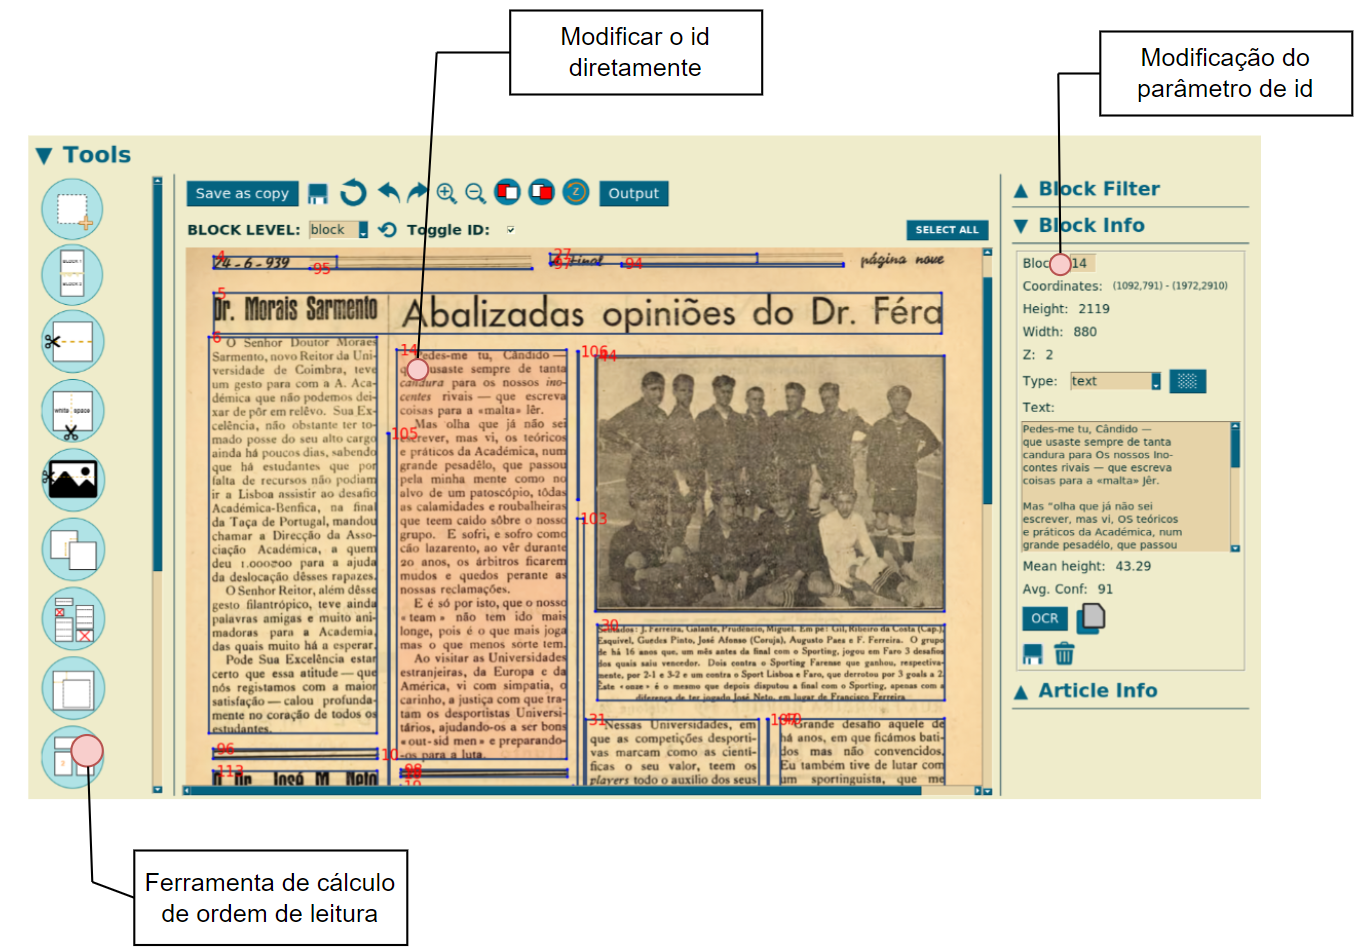
\includegraphics[width=0.7\textwidth]{images/ilustracoes/ocr_editor_change_block_id.png}
	\caption{OCR Editor: ordenação de blocos.}
	\label{fig:ocr_editor_change_block_id}
\end{figure}


\highlight{Segmentação de blocos em artigos}


Na pipeline, a segmentação da OCR Tree em artigos é uma das últimas operações realizadas, sendo o seu output extremamente dependente do sucesso das operações antecedentes. Novamente, a manipulação manual destes aparenta-se útil.

Uma aba específica para edição destes está presente no editor.

Várias operações estão relacionados com a manipulação de artigos:

\textbf{Segmentação da OCR Tree em artigos} utilizando o método semelhante ao discutido para a pipeline.


\textbf{Adicionar ou remover blocos de um artigo}, selecionando o artigo, o que irá atualizar a lista de blocos selecionados com os pertencentes ao artigo. Selecionar blocos não pertencentes ao artigo, no caso de se querer adicionar blocos; ou clicar em blocos dentro dos selecionados, para remover blocos do artigo. Por fim, atualiza-se o artigo para guardar as alterações.

\textbf{Adicionar um artigo}, ao selecionar bloco(s) e carregar para adicionar um artigo.


\textbf{Remover um artigo}, selecionando o artigo e clicando para o remover.

\textbf{Alterar ordem dos artigos}, ao selecionar um artigo e no botão para subir ou descer o seu lugar na ordem de artigos. Esta ordem tem influência na ordem em que os artigos aparecerão no output.

\begin{figure}[H]
	\centering
	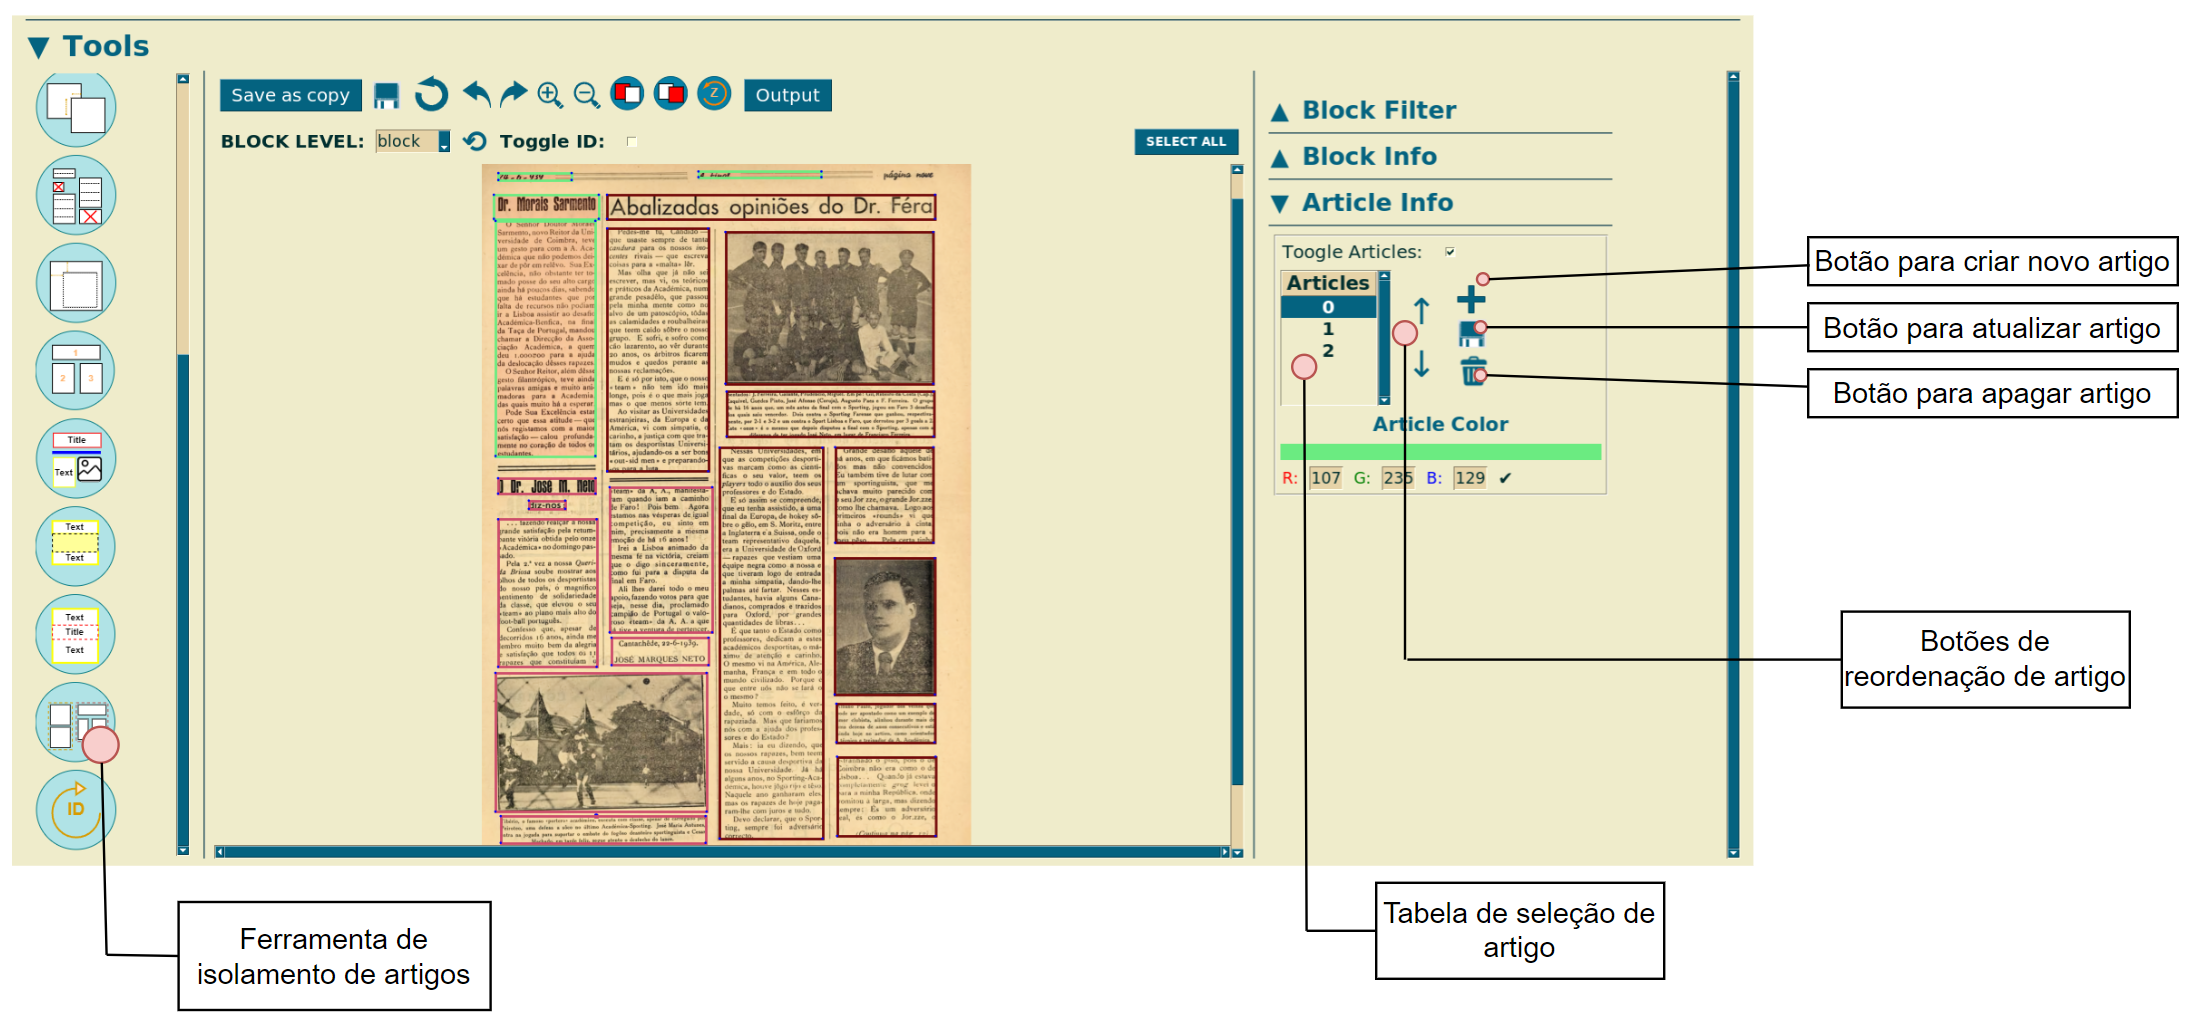
\includegraphics[width=0.9\textwidth]{images/ilustracoes/ocr_editor_articles.png}
	\caption{OCR Editor: manipulação de artigos.}
	\label{fig:ocr_editor_articles}
\end{figure}


\highlight{Divisão de imagem}

De forma a facilitar a criação de resultados OCR em locais específicos de uma imagem, foi implementada uma funcionalidade única para o OSDOCR Editor que possibilita o corte de uma imagem.

Esta funciona de forma semelhante ao corte de um bloco, onde será realizado um corte que será visualmente representado por uma linha.


Antes de o corte ser realizado, será questionado qual das partes da imagem se pretende manter.

Realizado o corte, uma nova imagem (recortada da original) será criada, e os nodos da OCR Tree inseridos na área recortada serão adicionados na OCR Tree correspondente a esta imagem. Realça-se que apenas os nodos que apresentem uma bounding box completamente dentro da área serão incluídos, sendo que será recorrente pedaços significativos de texto percam o seu respetivo bloco, no caso de este texto ter continuação numa área fora do recorte.

\begin{figure}[H]
	\centering
	\hspace*{-1.8cm}
	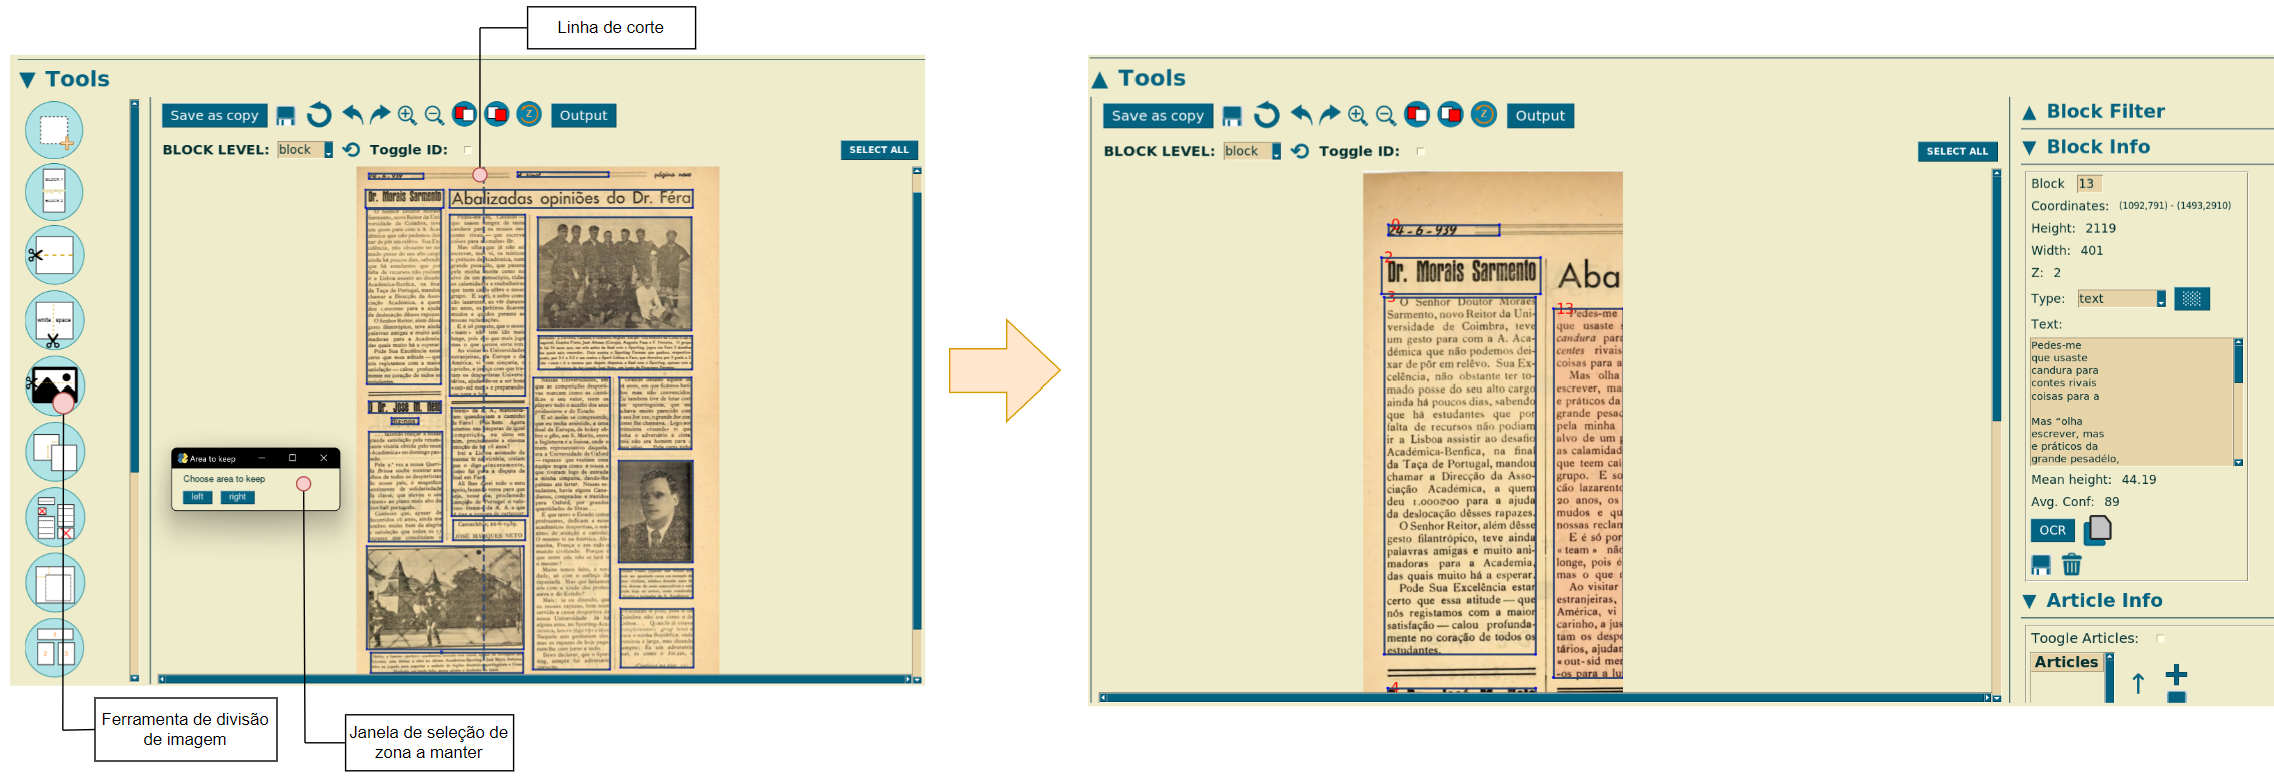
\includegraphics[width=1.2\textwidth]{images/ilustracoes/ocr_editor_split_image.png}
	\caption{OCR Editor: divisão de imagem.}
	\label{fig:ocr_editor_split_image}
\end{figure}



\subsection{Outputs}

O editor permite ainda a geração de outputs textuais semelhantes aos da pipeline. 

É possível a geração de ficheiros do tipo \textit{txt} ou \textit{markdown}, para documentos do tipo jornal - criando artigos caso não existam - ou simples. O tipo de documento pode ser modificado através das configurações do editor.

Este output textual é opcional, ao contrário da pipeline.

A OCR Tree utilizada como input será modificada - caso operações sob ela sejam aplicadas -, sendo portanto um output resultante da utilização do editor. 

Utilizando o método de divisão de imagem, o recorte da imagem também será também guardado como uma nova imagem, pareado com o respetivo ficheiro OCR Tree.


\begin{figure}[H]
	\centering
	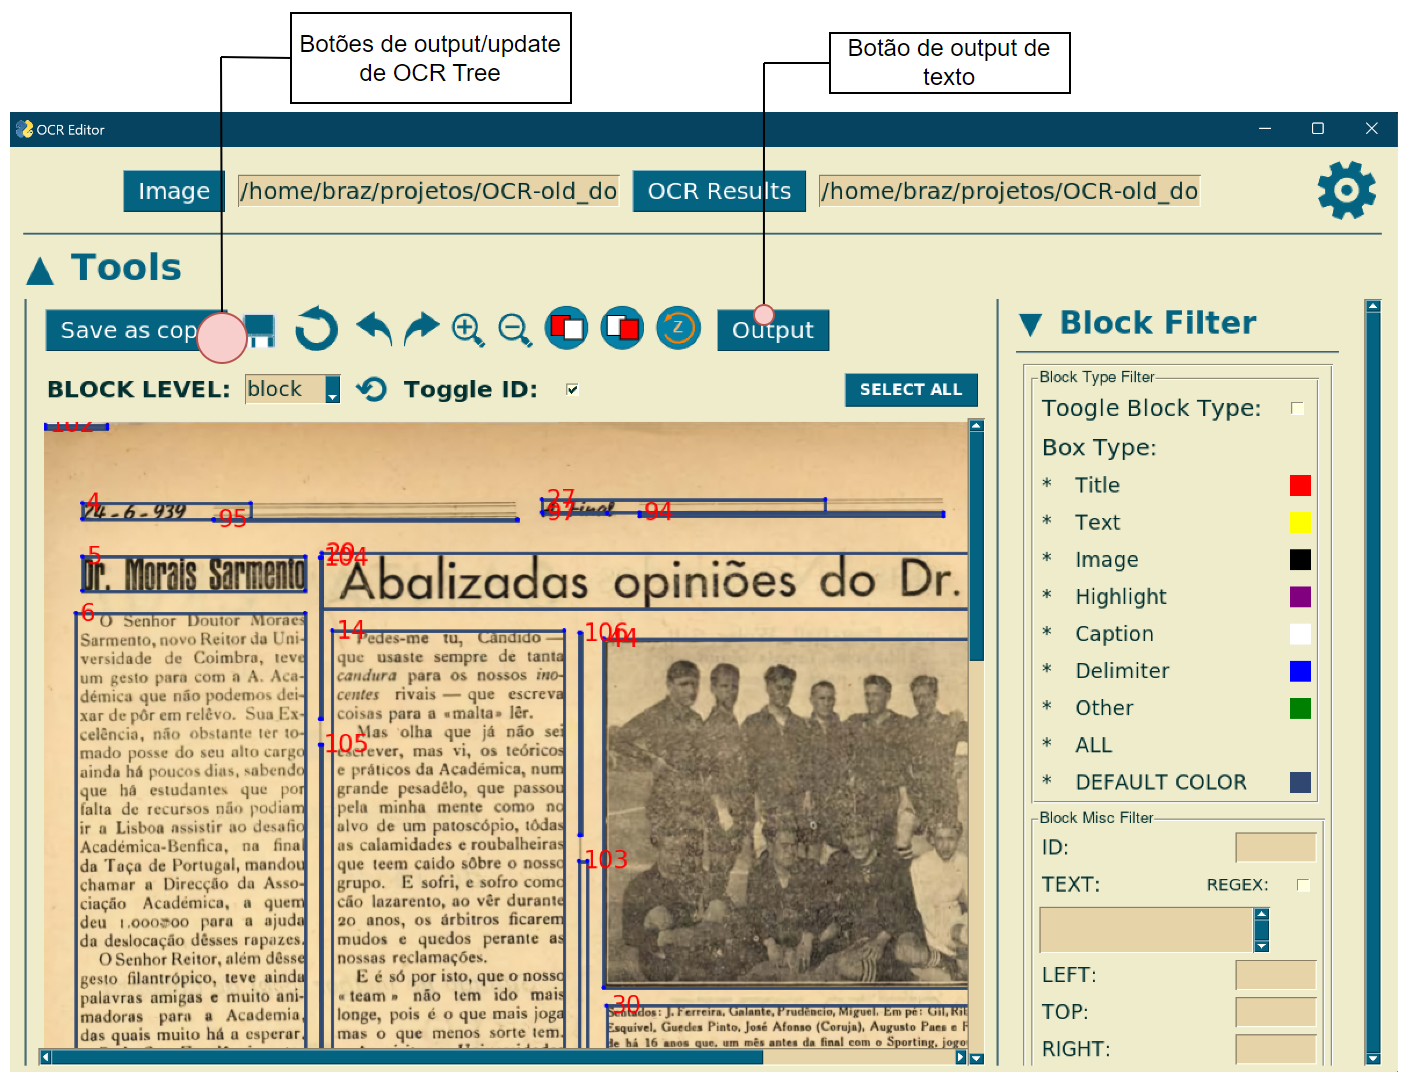
\includegraphics[width=0.6\textwidth]{images/ilustracoes/ocr_editor_output.png}
	\caption{OCR Editor: output.}
	\label{fig:ocr_editor_output}
\end{figure}


\subsection{Operações adicionais}

Serve esta última secção para descrever outras funcionalidades do editor, que se agrupam mais dentro de \textit{quality of life} ao invés de pura manipulação dos dados.

\highlight{Cache de operações}

Como na generalidade dos editores, este não é exceção na habilidade de retroceder e reconstruir operações. Tal permite desfazer ou refazer ações rapidamente, tornando o editor uma ferramenta ainda mais útil para a manipulação destes tipos de dados que podem ser consideravelmente densos.


Esta funcionalidade é possível através do uso de uma cache que vai sendo atualizada após a realização de cada operação.

O tamanho desta cache está por defeito definido para 10, mas pode ser alterado nas configurações do editor.


\highlight{Filtro de blocos}

A capacidade de filtragem em ferramentas de edição traz proveito para a sua utilização, através da permissão de maior controlo e focagem de conteúdos interessantes.

Exemplo disto é a existência de tipos essenciais para a criação de outputs especiais, como é o caso do "title" para a geração de artigos. A possibilidade para facilmente distinguir quais os blocos deste tipo existentes é essencial. 

De forma sucinta, os filtros disponíveis são:

\begin{itemize}\setlength\itemsep{-0.8em}
	\item Nível de bloco
	\item Tipo de bloco
	\item Id de bloco
	\item Texto de bloco
	\item Coordenadas de bloco
\end{itemize}



\highlight{Altura de blocos}

A disponibilização de um referencial de altura para os blocos permite a resolução de conflito entre blocos que se intersetam ou estão dentro de outros.

Nestes casos, se não houver distinção da altura entre estes, não será possível selecionar o pretendido entre os dois.

No entanto, selecionando um dos blocos e, alterando a sua altura, torna-se possível criar distinção entre os dois para mais facilmente selecionar aquele que anteriormente não era diretamente selecionável.



\highlight{Redimensionamento do input}

O editor permite ainda a realização de redimensionamento da imagem de input para facilitar a visualização e edição local da respetiva parte da OCR Tree nesta. A OCR Tree é automaticamente deslocada sempre que um redimensionamento ocorre.


\begin{figure}[H]
	\centering
	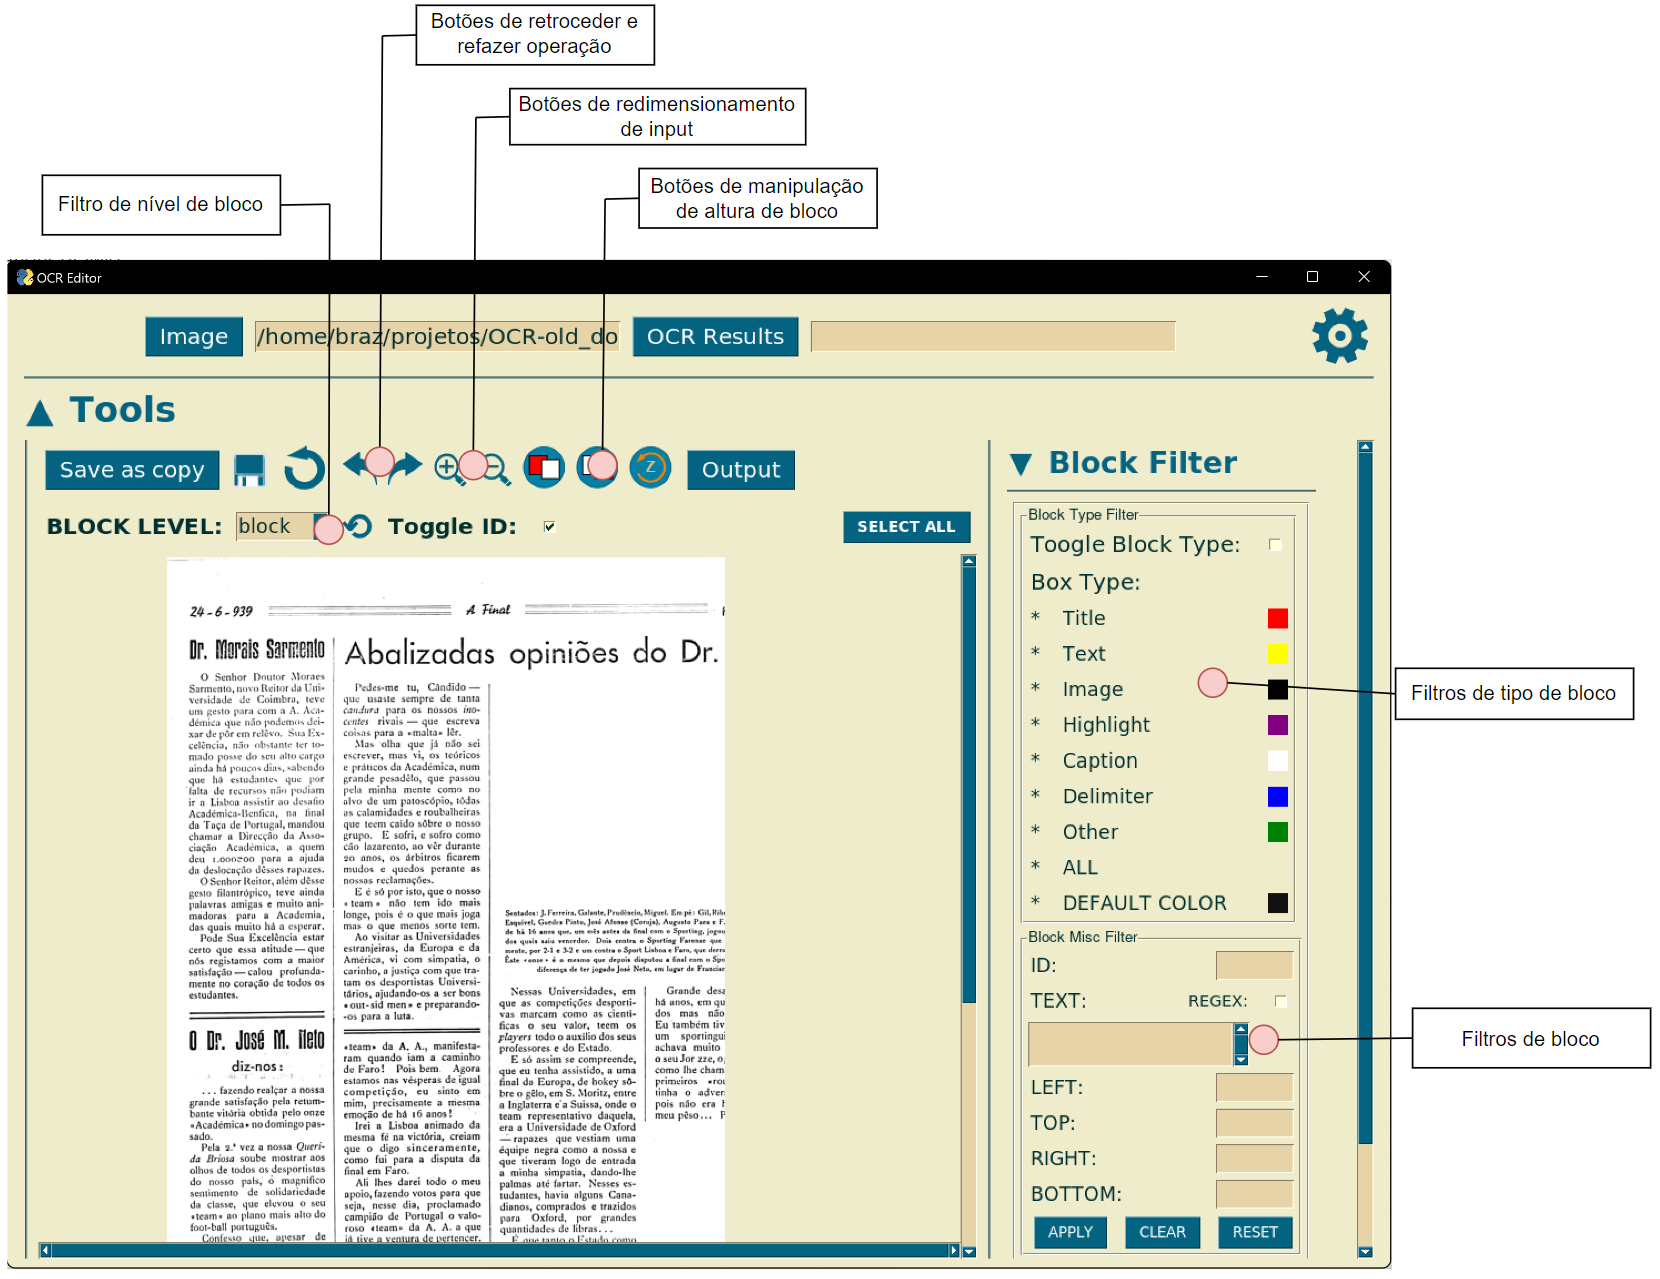
\includegraphics[width=0.9\textwidth]{images/ilustracoes/ocr_editor_aditional_operations.png}
	\caption{OCR Editor: operações adicionais.}
	\label{fig:ocr_editor_aditional_operations}
\end{figure}


\highlight{Configurações do editor}

De forma a poder alterar a utilização do editor, uma janela de configurações foi disponibilizada. Esta é composta por 3 abas principais: configurações gerais do editor; configurações das ferramentas; configurações da pipeline.

As \textbf{configurações gerais}, abrangem definições visuais do editor, como zoom inicial, cor e grossura das bounding boxes; e definições do output, como o formato, tipo e tratamento de texto.

As \textbf{configurações das ferramentas}, permitem modificar o comportamento de algumas das ferramentas, por exemplo: definir se no split de imagem, se mantém todas as caixas que intersetam ou estão dentro da zona escolhida, ou apenas as que estão completamente dentro.

As \textbf{configurações da pipeline}, são uma versão reduzida das configurações da OSDOCR Pipeline. Estas são na realidade também configurações de uma ferramenta mas, sendo a quantidade de opções considerável, torna-se mais simples para o utilizador ter uma janela dedicada a esta ferramenta.


\begin{figure}[H]
	\centering
	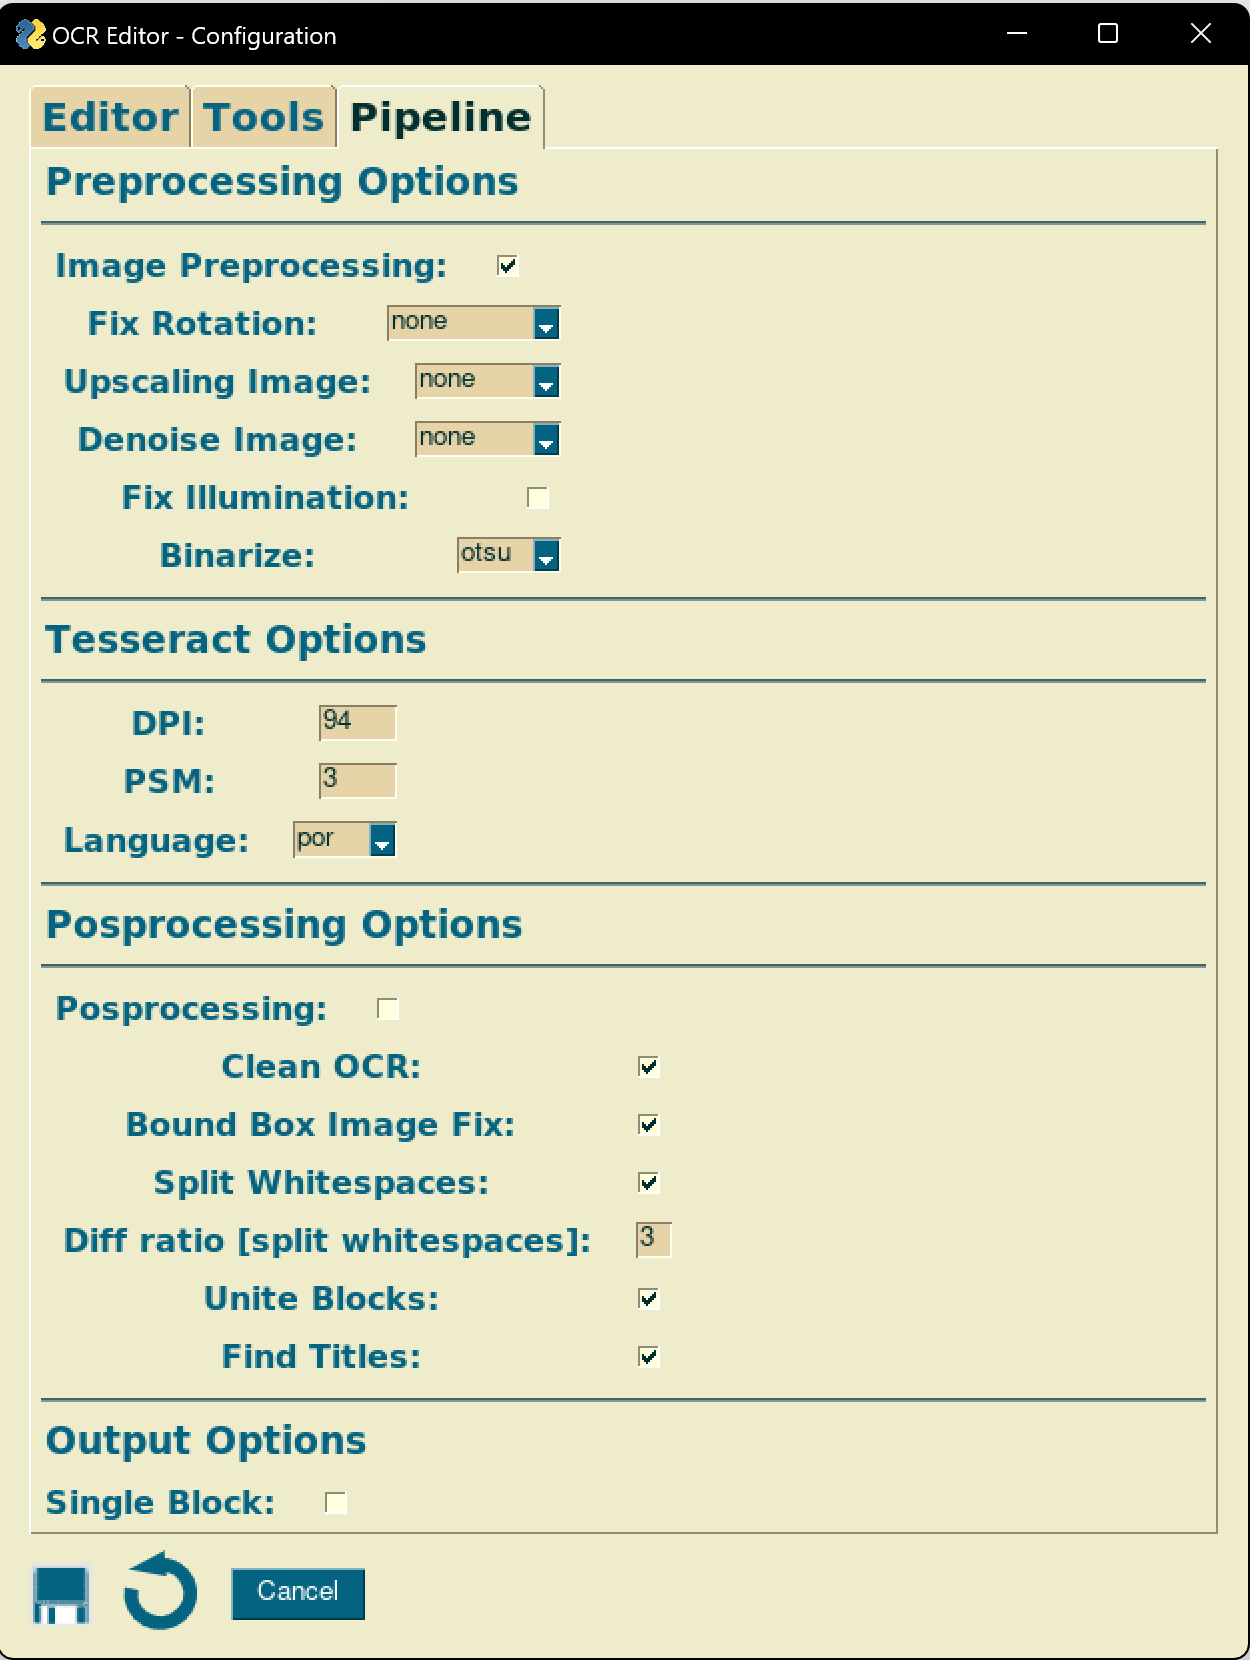
\includegraphics[width=0.4\textwidth]{images/ilustracoes/ocr_editor_configurations.png}
	\caption{OCR Editor: janela de configurações.}
	\label{fig:ocr_editor_configurations}
\end{figure}




% funcionalidades disponiveis
%% abir diferentes resultados OCR para uma mesma imagem
%% mover blocos singularmente ou em grupo
%% ajustar dimensoes de blocos
%% OCR de bloco
%%% configuracoes de OCR
%% configuracoes de editor
%% dividir bloco manualmente
%% dividir bloco por espaços vazios
%% categorizar blocos manualmente
%% ordenar blocos
%% calcular ordem de blocos
%% gerar artigos automaticamente
%% gerir artigos
%%% adicionar e remover
%%% adicionar e remover blocos a artigos
%%% alterar ordem dos artigos
%% gerar output
%%% simples
%%% markdown
%%% OCR Tree

%% cache de operacoes
%%% retroceder e reconstruir operacoes





